\documentclass[12pt, a4paper]{report}

% ---- Packages ----
\usepackage[utf8]{inputenc}
\usepackage[T1]{fontenc}
\usepackage{times}
\usepackage[margin=1in]{geometry}
\usepackage{setspace}
\usepackage{graphicx}
\graphicspath{{./figures/}{./}{images/}}
\DeclareGraphicsExtensions{.pdf,.png,.jpg,.jpeg}
\usepackage{tikz}
\usetikzlibrary{arrows.meta,positioning,shapes.geometric}
\usepackage{amsmath, amssymb}
\usepackage{natbib}
\usepackage{hyperref}
\usepackage{booktabs}
\usepackage{caption}
\usepackage{titlesec}
\usepackage{tocloft}
\usepackage{indentfirst}
\usepackage{parskip}

% ---- Formatting ----
\doublespacing
\setlength{\parindent}{1.27cm}
\setlength{\parskip}{0pt}

% Chapter/Section formatting
\titleformat{\chapter}[display]
  {\normalfont\bfseries\centering\Large}
  {CHAPTER \thechapter}{12pt}{\Large\MakeUppercase}
\titlespacing*{\chapter}{0pt}{-20pt}{20pt}

\titleformat{\section}
  {\normalfont\bfseries\large}
  {\thesection}{1em}{}

\titleformat{\subsection}
  {\normalfont\bfseries\normalsize}
  {\thesubsection}{1em}{}

\titleformat{\subsubsection}
  {\normalfont\bfseries\normalsize\itshape}
  {\thesubsubsection}{1em}{}

% TOC formatting
\renewcommand{\contentsname}{TABLE OF CONTENTS}
\renewcommand{\cftchapfont}{\bfseries}
\renewcommand{\cftsecfont}{\normalfont}

\hypersetup{
    colorlinks=true,
    linkcolor=black,
    citecolor=black,
    urlcolor=blue
}

% Load auto-generated numerical findings from main.py output.
% Run main.py first to produce results/results_summary.tex.
\InputIfFileExists{results/results_summary.tex}{}{}

\begin{document}

\hypersetup{pageanchor=false}

% ============================================================
% TITLE PAGE
% ============================================================

\begin{titlepage}
\thispagestyle{empty}
\begin{center}
\singlespacing

\vspace*{0.3cm}

\includegraphics[width=0.45\textwidth]{logo}

\vspace{0.9cm}

{\Large \textbf{A Coopetitive, Model-Agnostic Ensemble Weighting Framework via M\"{o}bius Decomposition: An Empirical Benchmark Study}}

\vspace{0.5cm}
\rule{0.75\textwidth}{0.4pt}

\vspace{0.9cm}

A Special Project Submitted to the

\vspace{0.2cm}
Faculty of the Department of Computer Science,

\vspace{0.2cm}
University of the Philippines Cebu

\vspace{0.7cm}

In Partial Fulfillment

\vspace{0.2cm}
of the Requirements for the Degree

\vspace{0.2cm}
Bachelor of Science in Computer Science

\vspace{0.6cm}
\rule{0.75\textwidth}{0.4pt}

\vfill

{\large \textbf{MAXELL G. MILAY}}\\
BS Computer Science

\vspace{0.6cm}

{\large \textbf{DHARRYL PRINCE ABELLANA}}\\
Special Problem Adviser

\vspace{0.6cm}

{\large \textbf{February 2026}}

\end{center}
\end{titlepage}


% ============================================================
% PERMISSION PAGE
% ============================================================
\clearpage
\thispagestyle{empty}
\begin{center}
\singlespacing

\vspace*{0.3cm}

\includegraphics[width=0.45\textwidth]{logo}

\vspace{0.6cm}

{\large \textbf{UNIVERSITY OF THE PHILIPPINES CEBU}}\\
{\large \textbf{College of Science}}\\
{\large \textbf{Department of Computer Science}}

\vspace{0.7cm}

{\large \textbf{A Coopetitive, Model-Agnostic Ensemble Weighting Framework via M\"{o}bius Decomposition: An Empirical Benchmark Study}}

\vspace{0.9cm}

\textbf{Permission is given for the following people to have access to this thesis:}

\vspace{0.5cm}

\begin{tabular}{|p{8.2cm}|p{3cm}|}
\hline
\textbf{Available to the general public} & \textbf{Yes} \\
\hline
\textbf{Available only after consultation with the author or thesis adviser} & \textbf{Yes} \\
\hline
\textbf{Available to those bound by a confidentiality agreement} & \textbf{Yes} \\
\hline
\end{tabular}

\vfill

{\large \textbf{MAXELL G. MILAY}}\\
Student

\vspace{0.8cm}

{\large \textbf{DHARRYL PRINCE ABELLANA}}\\
Special Problem Adviser

\end{center}

\newpage

% ============================================================
% TABLE OF CONTENTS
% ============================================================
\hypersetup{pageanchor=true}
\pagenumbering{arabic}
\tableofcontents
\newpage

% ============================================================
% CHAPTER 1: THE PROBLEM AND ITS SCOPE
% ============================================================
\chapter{The Problem and Its Scope}

\section{Rationale}

Ensemble methods represent one of the most effective strategies in machine learning for improving predictive performance by combining multiple base models. Despite their widespread adoption, a persistent and fundamental challenge remains: determining how much weight each constituent model should receive within the ensemble. Simple approaches such as equal weighting or performance-proportional weighting fail to account for the complex interdependencies among models, often resulting in suboptimal combinations where redundant models dilute the contributions of complementary ones \citep{kuncheva2003measures, demsar2006statistical}.

The Shapley value from cooperative game theory \citep{shapley1953value} offers a principled alternative by assigning each model a weight proportional to its average marginal contribution across all possible sub-ensembles. Recent work has established the promise of Shapley-based approaches in ensemble weighting and model valuation \citep{rozemberczki2021shapley, rozemberczki2022shapley, bimonte2024mortality}. However, the Shapley value has a structural limitation: because it averages each model's contribution over all coalition contexts, it entangles each model's standalone quality with its interaction effects relative to the other models in the pool. A model with modest standalone performance but strong complementarity with others may receive the same Shapley weight as one with high standalone performance but redundant interactions, with no way to distinguish the two cases from the Shapley weight alone. Practitioners who attempt to correct for this entanglement by augmenting Shapley values with the Shapley Interaction Index (SII) inadvertently introduce double-counting: the interaction information already embedded in the Shapley value is then attributed a second time through the additive SII terms, distorting the resulting weights. Three specific technical gaps arising from these limitations are formalized in \S\,1.2.

This study proposes a framework that resolves these gaps using the M\"{o}bius decomposition, also known as Harsanyi dividends \citep{harsanyi1959bargaining, harsanyi1963simplified}. The M\"{o}bius transform uniquely decomposes the characteristic function of the ensemble game into non-overlapping contributions---singleton dividends that capture each model's pure standalone value and pairwise dividends that capture the surplus or deficit arising exclusively from model interactions---and produces a pairwise dividend matrix that serves as an interpretable diagnostic, revealing which model pairs are complementary, redundant, or independent. Drawing on the concept of coopetition \citep{brandenburger1996coopetition}, the framework is termed ``coopetitive'' because the cooperative component (singleton dividends measuring standalone contribution) and the competitive component (negative pairwise dividends penalizing redundancy) are balanced through a tunable parameter $\lambda$. The proposed weighting formula is deliberately simple; its value lies not in computational sophistication but in providing a principled, interpretable mechanism for diagnosing and leveraging model interactions that more powerful but opaque methods like stacking do not offer. While the Shapley Interaction Index has been used extensively for feature-level attribution in explainable AI \citep{tsai2023faith, muschalik2024shapiq}, no prior work has applied the M\"{o}bius decomposition to construct ensemble weights that cleanly separate individual and interaction contributions. This study addresses that gap.

\section{Statement of the Problem}

The three gaps introduced in \S\,1.1 are articulated formally below. The first is the entanglement gap. The Shapley value \citep{rozemberczki2022shapley}, the most theoretically grounded approach to model valuation in ensembles, entangles individual and interaction effects into a single aggregate score. Specifically, because $\phi_i = \sum_{T \ni i} m(T)/|T|$, the Shapley value of model $i$ incorporates diluted versions of all interaction dividends involving $i$. This means that a model with modest standalone performance but strong complementarity with others may receive the same Shapley weight as one with high standalone performance but redundant interactions. The inability to disentangle these two dimensions prevents practitioners from understanding why a model receives a particular weight and limits the potential for targeted ensemble optimization.

The second is the double-counting gap. If practitioners attempt to correct for interactions by augmenting Shapley values with the Shapley Interaction Index, the resulting formulation $s_i = \phi_i + \lambda \sum_{j \neq i} \Delta_{ij}$ introduces systematic double-counting of pairwise effects. The interaction information already embedded within $\phi_i$ is counted again through the additive $\Delta_{ij}$ terms, distorting the resulting weights and undermining the theoretical guarantees of the approach. To the authors' knowledge, no established ensemble weighting method currently addresses this double-counting problem.

The third is the interpretability gap. Existing ensemble combination methods, including stacking and blending, optimize weights through cross-validated meta-learning. While individual model quality can often be assessed in isolation---for example, through standalone accuracy or the model's own Shapley value in the ensemble game---no standard ensemble method produces a pairwise diagnostic that reveals which specific model pairs are complementary, redundant, or independent within a given pool. Practitioners cannot determine from the ensemble weights alone how the interaction structure of the pool influenced the final combination, limiting the ability to diagnose ensemble behavior, guide model selection, and communicate results to stakeholders.

The M\"{o}bius decomposition directly resolves all three gaps by construction, as established in \S\,2.3.

\section{Research Objectives}

The primary objective of this research was to design and empirically evaluate a Coopetitive Model-Agnostic Ensembling Framework that uses the M\"{o}bius decomposition to construct ensemble weights from non-overlapping individual and interaction components. This overarching objective was operationalized through the following specific aims.

The first aim was to design a coopetitive weight formula that combines singleton Harsanyi dividends $m(\{i\})$, capturing each model's pure standalone contribution, with pairwise dividends $m(\{i,j\})$, capturing interaction effects, through a tunable parameter $\lambda$ that controls the trade-off between individual model quality and interaction structure. The formula $s_i = m(\{i\}) + \lambda\,\frac{1}{2}\sum_{j \neq i} m(\{i,j\})$ ensures non-overlapping accounting of individual and interaction information.

The second aim was to establish the construct validity of pairwise Harsanyi dividends as measures of model complementarity and redundancy through controlled experiments involving synthetic redundancy injection, monotonicity testing, correlation with established diversity metrics, and negative control conditions.

The third aim was to conduct a systematic ablation study that isolates the contribution of each component (individual dividends, interaction dividends, and their combination) by comparing equal weighting, performance-weighted weighting, individual-only ($\lambda = 0$), interaction-only, and full coopetitive variants across multiple benchmark datasets. Because the individual-only variant ($\lambda = 0$) is algebraically equivalent to performance-weighted weighting when AUC is the metric, this equivalence first serves as a sanity check; the ablation then tests whether the interaction term ($\lambda > 0$) adds value beyond this established baseline.

The fourth aim was to benchmark the coopetitive framework against established ensemble methods, including equal weighting, performance-weighted weighting, cooperative Shapley weighting, stacking with cross-validated logistic regression, and the best single model, using Friedman tests with Holm-corrected pairwise Wilcoxon post-hoc comparisons.

The fifth aim was to characterize the full sensitivity landscape of ensemble performance to the $\lambda$ parameter through a systematic sweep across $\lambda \in [0, 2.0]$, complementing the binary question of Aim 3 (whether $\lambda > 0$ helps) by mapping the shape and dataset-dependence of the performance--parameter curve, and to determine whether a fixed default value can achieve near-optimal performance across datasets.

\section{Significance of the Study}

This research holds significance for both the theoretical foundations of ensemble learning and the practical application of model combination strategies.

From a theoretical perspective, this study contributes to the body of knowledge by providing the first empirical evaluation of M\"{o}bius-based ensemble weighting that cleanly separates individual model quality from interaction structure. While the Shapley Interaction Index has been extensively studied in the context of feature attribution and explainable AI \citep{tsai2023faith, muschalik2024shapiq}, its application to ensemble weight construction has remained unexplored. By demonstrating that the non-overlapping property of Harsanyi dividends can serve as a principled foundation for ensemble combination, this study extends cooperative game theory's applicability within machine learning. The construct validity experiments characterize these relationships empirically; detailed findings are presented in \S\,3.5.1.

From a practical perspective, this research offers several contributions to practitioners and tool developers. For practitioners in data science and machine learning, the framework provides an interpretable diagnostic tool in the form of the pairwise dividend matrix, which reveals which model pairs are complementary, redundant, or independent. This information directly informs decisions about model selection, pool construction, and ensemble design. For researchers working on automated machine learning and ensemble selection, the coopetitive weight formula offers a computationally tractable alternative to stacking that does not require cross-validated meta-learning, making it suitable for scenarios where computational budgets are limited or where interpretability is a priority. For the broader machine learning community, the $\lambda$ sensitivity analysis provides practical guidance on default parameter selection, and the systematic comparison with established methods clarifies the conditions under which interaction-aware weighting offers meaningful improvements over simpler baselines.

It should be emphasized that this study does not claim that the coopetitive framework will necessarily outperform stacking in raw predictive accuracy. Rather, the contribution lies in offering a complementary tool that trades some potential performance for interpretability and diagnostic value. The empirical evaluation clarifies the magnitude of any performance trade-off and the conditions under which interaction-aware weighting provides meaningful improvements over simpler baselines.

\section{Scope and Delimitation}

This study focused on empirically evaluating the proposed coopetitive ensembling framework using a pool of five heterogeneous base models (Logistic Regression, Random Forest, Support Vector Machine with RBF kernel, XGBoost, and $k$-Nearest Neighbors) across multiple binary classification benchmark datasets. The evaluation followed a structured validation strategy comprising construct validity testing, ablation analysis, benchmark comparison, and sensitivity analysis, using AUC-ROC as the primary performance metric and negative Brier score as a secondary robustness check.

The framework was evaluated on fifteen binary classification datasets sourced from the OpenML benchmark suite and UCI repository, spanning medical, financial, socioeconomic, and scientific domains with sample sizes ranging from approximately 200 to 50,000. This expanded benchmark was designed to provide sufficient statistical power for the nonparametric tests used in the evaluation. The data splitting protocol followed a 60/20/20 train-validation-test partition for each dataset.

This research was specifically delimited in several respects. First, the M\"{o}bius decomposition was truncated to singleton and pairwise dividends only; higher-order interaction terms involving three or more models were excluded for parsimony. The decomposition coverage diagnostic quantifies how much of the total game value this truncation captures. Second, the framework was limited to pools of $n \leq 12$ models, as exact computation of all $2^n$ coalitions becomes impractical beyond this threshold. Third, the study used equal-weight probability averaging for coalition evaluation while applying non-equal coopetitive weights for the final ensemble. Fourth, the investigation focused exclusively on binary classification tasks and did not extend to multi-class classification or regression. Fifth, the base models used default or minimally tuned hyperparameters, as the focus of this study was on the weighting mechanism rather than on optimizing individual model performance. Finally, this research did not address real-time or streaming deployment scenarios, concentrating instead on the offline evaluation of ensemble weighting strategies.

\section{Definition of Terms}

To ensure clarity and a shared understanding of the concepts discussed in this study, the following terms are defined as they are used within this research context.

Ensemble method refers to any machine learning approach that combines the predictions of multiple base models to produce a single output. In this study, the ensemble combines five heterogeneous classifiers using weighted probability averaging, where the weights are derived from the proposed coopetitive framework.

Characteristic function, denoted $v(S)$, refers to a function that maps each coalition $S$ of base models to a performance score, specifically AUC-ROC, measured on a held-out validation set. The characteristic function forms the foundation of the cooperative game formulation that underlies the entire framework.

M\"{o}bius decomposition, also known as Harsanyi dividends, refers to the unique decomposition of the characteristic function $v(S)$ into non-overlapping contributions from subsets of models. Formally, $v(S) = \sum_{T \subseteq S} m(T)$, where each $m(T)$ is computed via the inclusion--exclusion formula $m(T) = \sum_{R \subseteq T} (-1)^{|T|-|R|} v(R)$.

Singleton dividend, denoted $m(\{i\})$, refers to the Harsanyi dividend for a single model $i$, computed as $m(\{i\}) = v(\{i\}) - v(\emptyset)$. This quantity captures the model's pure standalone contribution to the ensemble, with no interaction effects mixed in.

Pairwise dividend, denoted $m(\{i,j\})$, refers to the Harsanyi dividend for a pair of models, computed as $m(\{i,j\}) = v(\{i,j\}) - v(\{i\}) - v(\{j\}) + v(\emptyset)$. A positive pairwise dividend indicates complementarity between the two models, meaning their joint contribution exceeds the sum of their individual contributions. A negative dividend indicates redundancy, meaning the models overlap in predictive signal.

Coopetitive score, denoted $s_i$, refers to the combined score for model $i$ computed as $s_i = m(\{i\}) + \lambda\,\frac{1}{2}\sum_{j \neq i} m(\{i,j\})$, where $\lambda$ is the interaction weight parameter. This score integrates both individual quality and interaction structure into a single value from which the final ensemble weight is derived. Final ensemble weights are derived from $s_i$ via softmax normalization with an adaptive temperature parameter; see \S\,3.2.5.

Interaction weight $\lambda$ refers to the tunable parameter that controls the trade-off between individual model quality and interaction structure in the coopetitive score. When $\lambda = 0$, the framework reduces to pure performance-weighted weighting; as $\lambda$ increases, the weights become more sensitive to the complementarity and redundancy structure of the model pool.

Construct validity refers to the degree to which the pairwise Harsanyi dividends accurately measure the theoretical constructs of model complementarity and redundancy. This was established through controlled experiments with known ground truth, including synthetic redundancy injection and negative control conditions.

Shapley Interaction Index, denoted $\Delta_{ij}$, refers to the coalition-averaged measure of pairwise interaction between models $i$ and $j$, as defined by \citet{grabisch1999axiomatic}. Unlike the pairwise Harsanyi dividend, which evaluates interaction at the empty coalition only, the SII averages interactions across all possible coalition contexts. The context-sensitivity diagnostic compared these two measures.


% ============================================================
% CHAPTER 2: REVIEW OF RELATED LITERATURE
% ============================================================
\chapter{Review of Related Literature}

\section{Ensemble Methods and the Weighting Problem}

Ensemble methods have long been recognized as one of the most effective strategies for improving predictive performance in machine learning. The fundamental principle underlying all ensemble approaches is that combining diverse models can reduce variance, bias, or both, yielding predictions that are superior to any individual constituent model \citep{kuncheva2003measures}. Early approaches such as bagging \citep{breiman1996bagging} and boosting \citep{freund1997adaboost} demonstrated that even simple combination rules could yield substantial performance gains, and subsequent developments in stacking \citep{wolpert1992stacking} and blending introduced the idea of learning an optimal combination through a meta-learner trained on base model outputs.

Despite this progress, the question of how to optimally weight base models within an ensemble remains an active and unresolved area of research. The simplest strategy, equal weighting, treats all models as interchangeable regardless of their individual quality or their relationships with other models in the pool. Performance-proportional weighting assigns higher weights to models with better standalone accuracy, but this approach ignores the interaction structure of the ensemble entirely. A model with moderate standalone performance but strong complementarity with others will be systematically underweighted \citep{kuncheva2003measures}. Stacking with cross-validated meta-learners \citep{wolpert1992stacking} can implicitly capture some interaction effects, but the resulting weights are opaque and provide no interpretable information about model relationships: the meta-learner coefficients reflect how to combine outputs, not which model pairs are complementary or redundant. Ensemble pruning methods \citep{margineantu1997pruning}, which address the complementary problem of pool composition by selecting a subset of models rather than weighting all of them, offer a related perspective; the pairwise dividend matrix proposed in this study provides information directly applicable to such pruning decisions. This gap between the effectiveness of ensemble methods and the principled understanding of their combination dynamics motivates the application of game-theoretic concepts to ensemble weighting.

\section{Cooperative Game Theory in Machine Learning}

Cooperative game theory provides a natural mathematical framework for reasoning about the contributions of individual agents within a collective. The Shapley value \citep{shapley1953value}, the most widely studied solution concept, assigns each player a payoff proportional to their average marginal contribution across all possible coalitions. In the context of ensemble learning, each base model is treated as a player, and the characteristic function $v(S)$ maps each coalition of models to a performance metric evaluated on a held-out set \citep{rozemberczki2021shapley}.

Recent work has established the applicability of Shapley values to ensemble problems. \citet{rozemberczki2021shapley} formalized the ensemble weighting problem as a cooperative game and showed that Shapley-based weights could outperform equal weighting in several settings. \citet{rozemberczki2022shapley} extended this line of work by surveying the broader applications of the Shapley value in machine learning, including data valuation, feature attribution, and model selection. \citet{bimonte2024mortality} applied Shapley-based ensemble weighting to mortality forecasting models, demonstrating that cooperative game formulations could improve predictive accuracy in actuarial applications.

However, the standard Shapley value has a structural property that limits its usefulness for ensemble weight construction. As established by the M\"{o}bius representation \citep{harsanyi1959bargaining, dehez2017harsanyi}, the Shapley value can be written as $\phi_i = \sum_{T \ni i} m(T)/|T|$, where $m(T)$ are the Harsanyi dividends. This expression reveals that the Shapley value inherently mixes a model's standalone contribution $m(\{i\})$ with all higher-order interaction dividends involving model $i$, each diluted by the size of the respective subset. Consequently, practitioners cannot determine from the Shapley value alone whether a model's high weight is due to its strong standalone performance, its complementarity with other models, or some combination of both. This entanglement motivates the search for decomposition-based approaches that separate these two sources of value.

\section{The M\"{o}bius Decomposition and Harsanyi Dividends}

The M\"{o}bius decomposition, introduced in the context of cooperative games as Harsanyi dividends \citep{harsanyi1959bargaining, harsanyi1963simplified}, provides a unique decomposition of any characteristic function $v(S)$ into non-overlapping contributions from every subset of players. Formally, $v(S) = \sum_{T \subseteq S} m(T)$, where the dividends are computed via the inclusion--exclusion formula $m(T) = \sum_{R \subseteq T} (-1)^{|T|-|R|} v(R)$. The key property of this decomposition is that it is unique (see Theorem~1 in \citet{dehez2017harsanyi}): each coalition's surplus is assigned to exactly one subset $T$, with no term appearing in more than one place.

The M\"{o}bius decomposition has been applied in several domains beyond ensemble learning. In multicriteria decision making, it serves as the canonical representation of fuzzy measures (Choquet capacities), where singleton and pairwise dividends correspond to individual criterion importance and synergy between criteria \citep{grabisch1999axiomatic}. In explainable AI, higher-order Harsanyi dividends have been used to define interaction-aware feature attribution methods \citep{tsai2023faith, muschalik2024shapiq}. In cooperative game theory itself, the dividends underlie the definition of the Shapley value and related solution concepts \citep{dehez2017harsanyi}. However, none of these applications construct ensemble weights that explicitly separate individual model quality from pairwise interaction effects. The Shapley-based ensemble methods of \citet{rozemberczki2021shapley} and \citet{bimonte2024mortality} use the aggregate Shapley value, which entangles these two sources of value as noted above. The present study is, to the authors' knowledge, the first to apply the M\"{o}bius decomposition directly to ensemble weight construction with the explicit goal of non-overlapping separation of individual and interaction contributions.

For the purposes of ensemble weighting, the most relevant dividends are the singletons and pairs. The singleton dividend $m(\{i\}) = v(\{i\}) - v(\emptyset)$ captures the pure standalone contribution of model $i$, entirely free of interaction effects. The pairwise dividend $m(\{i,j\}) = v(\{i,j\}) - v(\{i\}) - v(\{j\}) + v(\emptyset)$ captures the surplus or deficit arising exclusively from the interaction between models $i$ and $j$, beyond their individual contributions. A positive pairwise dividend indicates that the two models are complementary, meaning their joint performance exceeds the sum of their individual performances, while a negative dividend indicates redundancy \citep{grabisch1999axiomatic}.

This non-overlapping property distinguishes the M\"{o}bius-based approach from formulations that combine Shapley values with interaction indices. In the latter case, the pairwise interaction information is counted twice: once within $\phi_i$ in diluted form, and once in the additive interaction term at full strength. The Harsanyi dividend framework avoids this entirely by construction, as the singleton and pairwise terms occupy separate, non-intersecting portions of the decomposition.

\section{The Shapley Interaction Index and Its Relationship to Harsanyi Dividends}

The Shapley Interaction Index (SII), as defined by \citet{grabisch1999axiomatic}, provides an alternative measure of pairwise interaction by averaging the discrete second-order difference of $v(S)$ over all possible coalition contexts. Formally, the SII $\Delta_{ij}$ computes the marginal interaction between models $i$ and $j$ conditional on every possible background coalition, then averages over all such backgrounds. The pairwise Harsanyi dividend $m(\{i,j\})$, by contrast, evaluates the interaction in isolation, considering only the empty coalition with no other models present.

This distinction has important practical implications. As the pool grows and coalition-dependent effects become more pronounced, the pairwise dividend and the SII may diverge. To the authors' knowledge, no prior study has systematically characterized this divergence in a classification ensemble context across varying pool sizes; this remains an open empirical question \citep{muschalik2024shapiq}. For the five-model pool evaluated in this study, the two measures were in close agreement ($r = 0.964$; see \S\,4.1.1), suggesting that the simpler Harsanyi-based measure is an adequate proxy in this setting. Recent work in explainable AI has made extensive use of the SII for feature-level attribution \citep{tsai2023faith, muschalik2024shapiq}, but no prior study has systematically compared pairwise Harsanyi dividends and the SII in the specific context of ensemble weight construction. The context-sensitivity diagnostic in this study addressed that gap by reporting the Spearman rank correlation between $m(\{i,j\})$ and $\Delta_{ij}$ for all model pairs, providing empirical evidence on when the simpler Harsanyi-based formulation is adequate.

\section{Diversity Measures in Ensemble Learning}

The concept of diversity among ensemble members has been studied extensively, as it is widely understood that combining diverse models yields better ensemble performance than combining similar ones. \citet{kuncheva2003measures} provided a comprehensive analysis of ten different diversity measures and their relationships with ensemble accuracy, concluding that no single measure perfectly predicts ensemble performance but that several, including the Q-statistic and the disagreement measure, capture meaningful aspects of model relationships.

The pairwise Harsanyi dividend $m(\{i,j\})$ offers a game-theoretic perspective on diversity that complements existing measures. Unlike the Q-statistic, which is defined purely in terms of the agreement or disagreement patterns of two classifiers on individual instances, the pairwise dividend is defined in terms of the coalition performance function and therefore directly reflects how the combination of two models affects the overall ensemble objective. It is hypothesized that pairwise dividends may capture aspects of model complementarity that instance-level diversity measures miss, particularly when model interactions are non-linear or dataset-dependent---a limitation that \citet{kuncheva2003measures} acknowledge for instance-level measures when predicting ensemble performance. This distinction is structural: instance-level measures are defined in terms of per-example prediction agreement between two classifiers, whereas the pairwise Harsanyi dividend is defined in terms of the coalition performance function and therefore reflects how combining two models affects the ensemble objective as a whole. The connection between these two perspectives on model diversity, and the extent to which game-theoretic interaction measures subsume or complement instance-level ones, remains empirically uncharacterized. The construct validity experiments in this study provide initial evidence on this question by comparing pairwise dividends directly against established diversity metrics.

\section{Limitations and Gaps in Existing Approaches}

Together, the literature reviewed in \S\S\,2.1--2.5 reveals that no existing work applies the M\"{o}bius decomposition directly to ensemble weight construction, that the double-counting problem arising from augmenting Shapley values with the SII has not been addressed in the ensemble weighting literature, and that the relationship between game-theoretic pairwise interaction measures and established instance-level diversity metrics remains empirically uncharacterized. The present study addresses these gaps through the coopetitive weight formula, construct validity experiments comparing pairwise dividends against established diversity measures, and a systematic ablation and benchmark evaluation with appropriate statistical methodology.

% ============================================================
% CHAPTER 3: METHODOLOGY
% ============================================================
\chapter{Methodology}

\section{Research Design}

This chapter presents the methodology for designing, implementing, and evaluating the Coopetitive Model-Agnostic Ensembling Framework for binary classification tasks. The study employed a comparative experimental design in which the independent variable was the ensemble weighting strategy and the dependent variable was the predictive performance measured by AUC-ROC and negative Brier score on held-out test sets. The research followed a structured four-phase validation strategy: construct validity testing, ablation analysis, benchmark comparison, and sensitivity analysis. Each phase built upon the results of the preceding phase, with construct validity serving as a prerequisite gate for all subsequent experiments.

The overall architecture of the proposed framework implements a pipeline that begins with a pool of heterogeneous base models, evaluates all possible coalitions on a validation set, computes M\"{o}bius dividends, derives coopetitive weights via the tunable formula, and produces a final weighted ensemble prediction. Figure~\ref{fig:research_design} illustrates the end-to-end flow of the study from data preparation through final evaluation.

\begin{figure}[htbp]
\centering
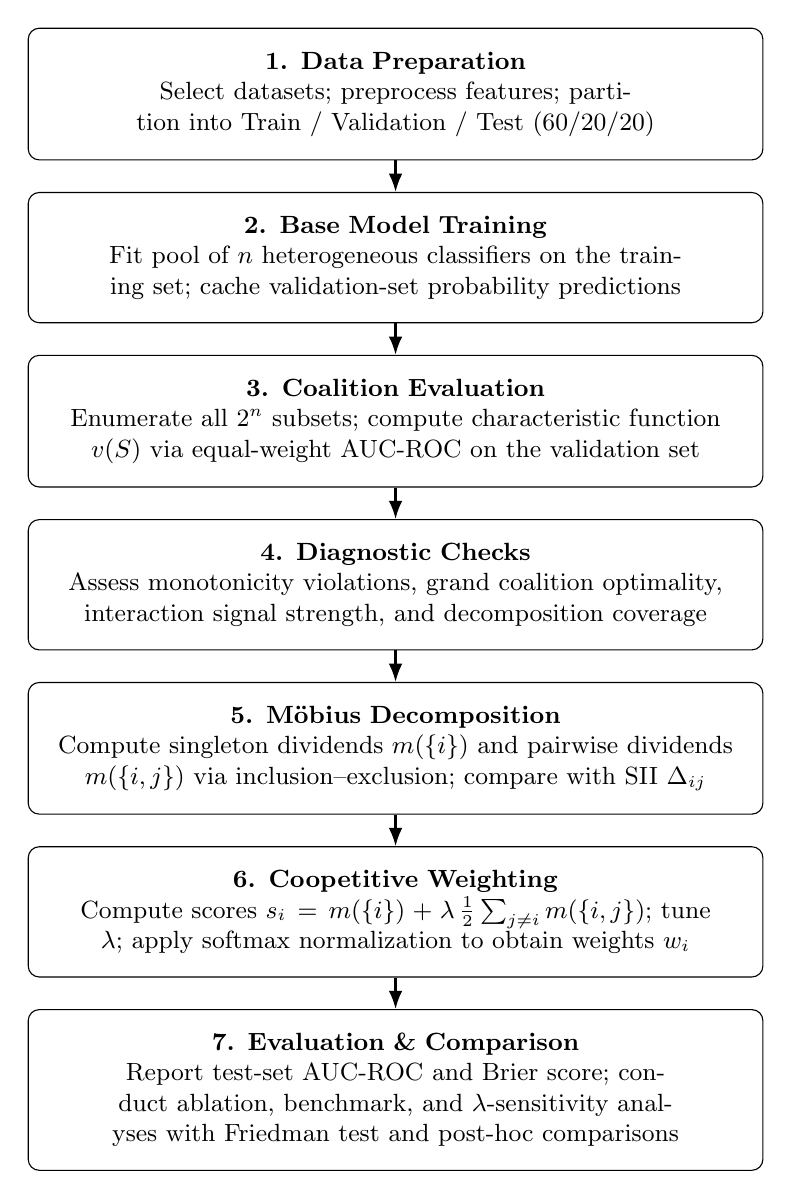
\begin{tikzpicture}[font=\small,
  block/.style={draw, rounded corners, align=center, text width=0.72\textwidth, minimum height=10mm, inner sep=3mm},
  line/.style={-Latex, thick},
  node distance=4mm]
\node[block] (P1) {\textbf{1. Data Preparation}\\
  Select datasets; preprocess features; partition into Train / Validation / Test (60/20/20)};
\node[block, below=of P1] (P2) {\textbf{2. Base Model Training}\\
  Fit pool of $n$ heterogeneous classifiers on the training set; cache validation-set probability predictions};
\node[block, below=of P2] (P3) {\textbf{3. Coalition Evaluation}\\
  Enumerate all $2^n$ subsets; compute characteristic function $v(S)$ via equal-weight AUC-ROC on the validation set};
\node[block, below=of P3] (P4) {\textbf{4. Diagnostic Checks}\\
  Assess monotonicity violations, grand coalition optimality, interaction signal strength, and decomposition coverage};
\node[block, below=of P4] (P5) {\textbf{5. M\"{o}bius Decomposition}\\
  Compute singleton dividends $m(\{i\})$ and pairwise dividends $m(\{i,j\})$ via inclusion--exclusion; compare with SII $\Delta_{ij}$};
\node[block, below=of P5] (P6) {\textbf{6. Coopetitive Weighting}\\
  Compute scores $s_i = m(\{i\}) + \lambda\,\tfrac{1}{2}\sum_{j\neq i}m(\{i,j\})$; tune $\lambda$; apply softmax normalization to obtain weights $w_i$};
\node[block, below=of P6] (P7) {\textbf{7. Evaluation \& Comparison}\\
  Report test-set AUC-ROC and Brier score; conduct ablation, benchmark, and $\lambda$-sensitivity analyses with Friedman test and post-hoc comparisons};
\draw[line] (P1) -- (P2);
\draw[line] (P2) -- (P3);
\draw[line] (P3) -- (P4);
\draw[line] (P4) -- (P5);
\draw[line] (P5) -- (P6);
\draw[line] (P6) -- (P7);
\end{tikzpicture}
\caption{End-to-end flow of the Coopetitive Ensembling Framework evaluation, organized by logical phase.}
\label{fig:research_design}
\end{figure}

\section{Formal Hypotheses}

The study tested the following formal hypotheses. The first hypothesis (H1) states that the coopetitive ensemble ($\lambda > 0$) achieves a higher mean AUC-ROC than the individual-only baseline ($\lambda = 0$) across benchmark datasets, indicating that the interaction term contributes positively to ensemble performance. The second hypothesis (H2) states that the pairwise Harsanyi dividends correctly identify known redundancy and complementarity structures in controlled experiments, as measured by sign consistency with injected ground truth. The third hypothesis (H3) states that the coopetitive framework achieves competitive or superior performance compared to established ensemble methods, including cooperative Shapley weighting and stacking, as assessed by Friedman test rankings across datasets. The fourth hypothesis (H4) states that a fixed default value of $\lambda$ achieves at least 95\% of the performance gain attainable by cross-validated $\lambda$ optimization, indicating practical robustness to parameter selection.

Note that H1 represents the single most important test in this study. Because the individual-only variant ($\lambda = 0$) is algebraically equivalent to performance-weighted weighting (since $m(\{i\}) = v(\{i\}) - v(\emptyset)$ and $v(\emptyset)$ is constant across models), the entire contribution of the interaction term rests on whether $\lambda > 0$ improves upon this simple baseline. Fundamentally, the study tests whether pairwise M\"{o}bius dividends add value beyond performance-weighted ensembling.

\section{Phase 1: Base Model Pool and Dataset Curation}

\subsection{Base Model Pool}

The framework required models from different algorithm families so that pairwise dividends would have meaningful complementarity structure to detect. A pool of $n = 5$ heterogeneous models served as the primary configuration. The pool comprised Logistic Regression (LR) with $\text{max\_iter} = 1000$, Random Forest (RF) with $\text{n\_estimators} = 200$, Support Vector Machine with RBF kernel (SVM) with $\text{probability} = \text{True}$, XGBoost (XGB) with $\text{n\_estimators} = 200$, and $k$-Nearest Neighbors (KNN) with $\text{n\_neighbors} = 7$. These five models span five distinct inductive biases (linear, bagging ensemble, kernel, boosting ensemble, and instance-based), and this diversity was expected to produce variation in the magnitude and sign of pairwise dividends. All models support \texttt{predict\_proba()} for probability output, which is required for the weighted probability averaging used in coalition evaluation.

In addition to the heterogeneous pool, a homogeneous pool of five tree-based variants was constructed for construct validity testing: RF(100), RF(200), RF(500), XGB(100), and XGB(200). These were expected to produce mostly negative pairwise dividends due to high redundancy, providing a controlled comparison against the heterogeneous pool.

\subsection{Dataset Selection}

To ensure adequate statistical power for nonparametric tests across methods, the framework was evaluated on fifteen binary classification benchmark datasets sourced from the OpenML benchmark suite and the UCI repository. The datasets were selected to span multiple domains and a range of sample sizes. Table~\ref{tab:datasets} summarizes the selected datasets.

\begin{table}[htbp]
\centering
\caption{Benchmark datasets for the empirical evaluation.}
\label{tab:datasets}
\begin{tabular}{llrl}
\toprule
\textbf{Dataset} & \textbf{Domain} & \textbf{Samples} & \textbf{Source} \\
\midrule
Breast Cancer Wisconsin & Medical & 569 & sklearn / UCI \\
Heart Disease (Cleveland) & Medical & 303 & UCI / OpenML \\
Pima Indians Diabetes & Medical & 768 & UCI / OpenML \\
Ionosphere & Physics / Signal & 351 & UCI / OpenML \\
German Credit & Financial & 1,000 & UCI / OpenML \\
Adult Census & Socioeconomic & 48,842 & UCI / OpenML \\
Australian Credit & Financial & 690 & UCI / OpenML \\
Sonar & Signal & 208 & UCI / OpenML \\
SPECT Heart & Medical & 267 & UCI / OpenML \\
Haberman Survival & Medical & 306 & UCI / OpenML \\
Banknote Authentication & Forensic & 1,372 & UCI / OpenML \\
Blood Transfusion & Medical & 748 & UCI / OpenML \\
Tic-Tac-Toe Endgame & Game / Logic & 958 & UCI / OpenML \\
Climate Model Crashes & Climate / Physics & 540 & UCI / OpenML \\
Phoneme & Signal & 5,404 & OpenML \\
\bottomrule
\end{tabular}
\end{table}

This selection spans medical, financial, socioeconomic, physics, forensic, and signal processing domains with sample sizes ranging from 208 to 48,842. The use of fifteen datasets provides substantially more statistical power for the Friedman test and post-hoc comparisons than the minimum of six recommended by \citet{demsar2006statistical}, reducing the risk of Type II errors in the benchmark comparison.

\subsection{Data Splitting Protocol}

For each dataset, the data were partitioned into three subsets: 60\% for training, 20\% for validation, and 20\% for testing. The training set was used exclusively for fitting the base models. The validation set was used for computing the characteristic function $v(S)$, M\"{o}bius dividends, and coopetitive weights, as well as for tuning the $\lambda$ parameter via inner cross-validation. The test set was held out entirely and used only for final reporting of ensemble performance, ensuring that the evaluation was unbiased by any information used during weight construction.

\section{Phase 2: Characteristic Function Evaluation and M\"{o}bius Decomposition}

\subsection{Coalition Evaluation}

For each dataset, the characteristic function $v(S)$ was computed for every coalition $S \subseteq N$, where $N = \{M_1, M_2, \ldots, M_5\}$. With $n = 5$ models, this required evaluating $2^5 = 32$ coalitions. Each coalition was evaluated by averaging the predicted probabilities of its constituent models with equal weights and computing the AUC-ROC of the resulting combined prediction on the validation set. Because model predictions were cached as arrays, each coalition evaluation reduced to array indexing and averaging, making exact computation tractable.

\subsection{Characteristic Function Diagnostics}

Before interpreting M\"{o}bius dividends, the characteristic function was subjected to four diagnostics with decision rules. The first diagnostic assessed the monotonicity violation rate by checking whether marginal contributions were predominantly positive; if more than 40\% of marginal contributions were negative, offending models were flagged and results were reported both with and without them, rather than silently removing them (which would introduce selection bias). The second diagnostic verified grand coalition optimality by checking whether $v(N)$ achieved the highest coalition value; if not, the study proceeded but reported the optimal coalition. The third diagnostic assessed the interaction signal by checking whether any pairwise dividends exceeded 0.001 in absolute value; if all were below this threshold, $\lambda$ was set to zero since the pairwise dividends would provide no meaningful signal. The fourth diagnostic assessed decomposition coverage by computing the proportion of $v(N) - v(\emptyset)$ captured by singleton and pairwise dividends alone; if coverage fell below 80\%, the study acknowledges that higher-order interactions are substantial and discusses this as a limitation.

\subsection{M\"{o}bius Dividend Computation}

The M\"{o}bius dividends were computed using the inclusion--exclusion formula. Singleton dividends were computed as $m(\{i\}) = v(\{i\}) - v(\emptyset)$ for each model $i$. Pairwise dividends were computed as $m(\{i,j\}) = v(\{i,j\}) - v(\{i\}) - v(\{j\}) + v(\emptyset)$ for each pair $(i, j)$ with $i \neq j$. Higher-order dividends for $|T| \geq 3$ were excluded from the current framework for parsimony. The decomposition coverage diagnostic quantifies the impact of this exclusion.

\subsection{Context-Sensitivity Diagnostic}

The Shapley Interaction Index $\Delta_{ij}$ was computed for all model pairs using the \texttt{shapiq} library. The Spearman rank correlation between $m(\{i,j\})$ and $\Delta_{ij}$ across all pairs was reported. If $r > 0.85$, the empty-coalition evaluation underlying the pairwise dividend was deemed an adequate proxy for the coalition-averaged interaction, justifying the simpler Harsanyi-based formulation. If $r < 0.70$, the pairwise dividends may not reliably represent the interaction structure within the full pool, and this was acknowledged as a limitation. Any pair exhibiting opposite signs for $m(\{i,j\})$ and $\Delta_{ij}$ was reported, as this would indicate that coalition context substantially alters the nature of the interaction.

\subsection{Coopetitive Weight Derivation}

The coopetitive score for each model $i$ was computed as $s_i = m(\{i\}) + \lambda\,\frac{1}{2}\sum_{j \neq i} m(\{i,j\})$. The factor of $\frac{1}{2}$ distributes each pairwise dividend equally between the two models involved, following the Shapley sharing rule within the Harsanyi set framework \citep{dehez2017harsanyi}. To convert scores to valid probability weights, a softmax normalization was applied: $w_i = \exp(s_i/\tau) / \sum_k \exp(s_k/\tau)$, where $\tau$ is a temperature parameter set to the standard deviation of the coopetitive scores. When all coopetitive scores are nearly identical, $\tau$ approaches zero; a floor of $\tau_{\min} = 10^{-6}$ was applied in practice to prevent numerical instability in this edge case. This formulation avoids the hard clamping of negative scores to zero (which can produce degenerate zero-weight assignments for models with high singleton dividends but large negative interaction sums) while still ensuring that models with lower coopetitive scores receive proportionally lower weights. The normalization scheme (softmax with adaptive temperature) was not experimentally compared against clamping-then-normalizing; this is acknowledged as an unvalidated design choice in \S\,3.9.

\subsection{Rank-Stability Diagnostic}

After computing coopetitive weights, the study recomputed $v(S)$ using those weights for aggregation rather than equal weights, then recomputed singleton dividends under the new characteristic function, and checked whether the ranking of models changed. The Spearman rank correlation between the original and recomputed individual dividends was reported. If $r > 0.90$, the ranking-preservation assumption underlying the equal-weight coalition evaluation was considered validated.

\section{Phase 3: Validation Experiments}

\subsection{Experiment 1: Construct Validity of Pairwise Dividends}

This experiment verified that pairwise Harsanyi dividends detect complementarity and redundancy when the ground truth is known, serving as a prerequisite gate for all subsequent experiments.

Test A was a controlled redundancy experiment. The procedure involved training a Random Forest model $M_1$, creating near-copies $M_2$ and $M_3$ by adding Gaussian noise with $\sigma = 0.01$ to $M_1$'s predictions, training different models $M_4$ (Logistic Regression) and $M_5$ (SVM), and computing all ten pairwise dividends. The primary pass criterion required that dividends among the near-copies ($m(\{1,2\}), m(\{1,3\}), m(\{2,3\})$) be more negative than dividends between dissimilar models ($m(\{1,4\}), m(\{1,5\}), m(\{4,5\})$), reflecting the framework's ability to distinguish more-redundant pairs from less-redundant ones. An initial criterion requiring dissimilar-model dividends to be positive or near-zero was revised after observing that strong classifiers on tabular data produce universally negative dividends even across algorithm families (see \S\,4.1.1 for the rationale and empirical evidence). Because this criterion change was informed by observed data rather than pre-specified theory, the Test A pass verdict should be treated as provisional: it holds under the revised relative-magnitude criterion, but replication with this criterion stated a priori is needed to fully establish the finding.

Test B assessed the correlation of pairwise dividends with existing diversity metrics and the context-sensitivity of the measures. The study computed $m(\{i,j\})$ alongside the Q-statistic \citep{kuncheva2003measures}, the disagreement measure, and the SII $\Delta_{ij}$ for all model pairs. Spearman rank correlations were reported for each pairing. The expected outcome was moderate-to-strong agreement, with the Spearman correlation between $m(\{i,j\})$ and $\Delta_{ij}$ serving as the critical context-sensitivity diagnostic.

Test C assessed monotonicity under increasing redundancy. A blended model $M_\alpha = (1-\alpha)M_a + \alpha M_b$ was created for $\alpha \in \{0, 0.1, \ldots, 1.0\}$, where $M_a$ is Logistic Regression and $M_b$ is Random Forest. The pass criterion required a Spearman correlation between $\alpha$ and $m(\{b, \alpha\})$ of less than $-0.9$, confirming that increasing similarity between models is monotonically reflected in increasingly negative pairwise dividends.

Test D was a negative control using independent error models. Using accuracy instead of AUC-ROC as $v(S)$ to avoid spurious rank-induced interactions, the pass criterion required all $|m(\{i,j\})| < 0.01$ and the mean absolute pairwise dividend to be at least five times smaller than in Test A.

\subsection{Experiment 2: Ablation Study}

This experiment isolated the contribution of each framework component and constituted the single most important experiment in the validation strategy. Six primary weighting variants were compared across all benchmark datasets. The equal-weight variant assigned $w_i = 1/n$ to each model. The performance-weighted variant assigned $w_i \propto \text{AUC}_i - 0.5$. The individual-only variant ($\lambda = 0$) assigned $w_i = m(\{i\}) / \sum m(\{j\})$, which is algebraically equivalent to the performance-weighted variant when AUC is the metric; this equivalence was verified as a sanity check. The interaction-only variant assigned $w_i \propto \max(\frac{1}{2}\sum m(\{i,j\}), 0)$, testing whether complementarity structure alone is sufficient for effective weighting. The coopetitive variant with fixed $\lambda = 0.5$ applied the full M\"{o}bius formula to test whether combining both individual and interaction terms outperforms either alone. The coopetitive variant with cross-validated $\lambda$ optimized $\lambda$ via 5-fold inner cross-validation on the validation set, searching over $\lambda \in \{0, 0.1, 0.2, \ldots, 2.0\}$ and selecting the value that maximizes mean AUC-ROC across folds, providing the practical upper bound.

Two additional variants were included to directly test the central theoretical claim of this study. The cooperative Shapley variant assigned $w_i = \phi_i / \sum \phi_j$, providing a baseline for the standard Shapley-based approach. The Shapley coopetitive variant assigned $s_i = \phi_i + \lambda \sum_{j \neq i} \Delta_{ij}$---the double-counting formula that this study argues is theoretically unsound. An a priori contrast between the M\"{o}bius-based coopetitive variant and the Shapley coopetitive variant was pre-specified as a direct test of whether the non-overlapping property of Harsanyi dividends matters in practice. If the M\"{o}bius-based variant outperforms the Shapley coopetitive variant, this demonstrates that avoiding double-counting helps; if the two are similar, the M\"{o}bius formulation is still preferred on theoretical grounds.

Replication was conducted with $k = 5$ random seeds per dataset. The ideal ordering of variant performance was: equal $<$ interaction-only $<$ individual-only $<$ coopetitive ($\lambda = 0.5$) $\leq$ coopetitive ($\lambda = \text{CV}$). The critical comparison between coopetitive and individual-only variants was tested as an a priori contrast at $\alpha = 0.05$, exempt from multiplicity correction following the recommendations of \citet{demsar2006statistical}. All remaining comparisons used Holm--Bonferroni correction. Effect sizes were reported as $r = Z/\sqrt{N}$ alongside $p$-values.

\subsection{Experiment 3: Benchmark Comparison}

The coopetitive framework was compared against five established ensemble methods: equal weighting with $w_i = 1/n$, performance-weighted weighting with $w_i \propto \text{AUC}_i - 0.5$, cooperative Shapley weighting with $w_i = \phi_i / \sum \phi_j$, stacking with a cross-validated logistic regression meta-learner, and the best single model selected on the validation set. Statistical significance was assessed using the Friedman test with Holm-corrected pairwise Wilcoxon post-hoc comparisons, following the methodology recommended by \citet{demsar2006statistical}. A critical difference diagram was produced using the \texttt{scikit-posthocs} library to visualize the average rank of each method and the significance groups.

It should be noted that even if the coopetitive framework shows only modest performance gains over the baselines, the pairwise dividend matrix provides interpretable diagnostics about model complementarity and redundancy that stacking and other opaque methods do not offer. This interpretability benefit was discussed alongside the quantitative results.

\subsection{Experiment 4: \texorpdfstring{$\lambda$}{lambda} Sensitivity Analysis and Factorial Interaction}

The sensitivity of ensemble performance to the $\lambda$ parameter was characterized by sweeping $\lambda \in [0, 2.0]$ in steps of 0.1 across all datasets. The analysis reported the optimal $\lambda^*$ mean and standard deviation across datasets, the performance loss incurred by using a fixed $\lambda = 0.5$ instead of the dataset-specific optimum, and the robustness ratio defined as the proportion of $\lambda$ values achieving at least 95\% of the maximum gain.

To provide a more nuanced understanding of the interaction between the $\lambda$ parameter and dataset characteristics, a two-factor analysis was conducted using a factorial ANOVA design. The two factors were the $\lambda$ level (treated as a discrete factor with levels corresponding to each sweep value) and the dataset identity. The factorial ANOVA tested for a significant main effect of $\lambda$, a significant main effect of dataset, and critically, a significant $\lambda \times \text{dataset}$ interaction effect. A significant interaction effect would indicate that the optimal $\lambda$ varies meaningfully across datasets, reinforcing the importance of the cross-validation-based tuning strategy. Conversely, a non-significant interaction would suggest that a single fixed $\lambda$ performs comparably across datasets, supporting the practical convenience of a default setting. The interaction pattern was visualized using an interaction plot showing the mean AUC-ROC at each $\lambda$ level for each dataset. This factorial analysis complemented the univariate sensitivity sweep by providing a statistically rigorous assessment of whether $\lambda$ sensitivity is dataset-dependent.

\section{Phase 4: Evaluation and Statistical Analysis}

\subsection{Primary Evaluation Metrics}

The primary evaluation metric was AUC-ROC, which measures the overall discriminatory ability of the ensemble across all classification thresholds. This metric is appropriate for binary classification tasks and is robust to class imbalance \citep{fawcett2006roc}. As a secondary robustness check, the negative Brier score was computed, which measures the calibration quality of the probabilistic predictions. Results were reported as mean $\pm$ standard deviation across five random seeds.

\subsection{Statistical Treatment}

The statistical analysis followed the methodology recommended by \citet{demsar2006statistical} for comparing classifiers over multiple datasets. For comparisons involving multiple methods, the Friedman test was applied first as a non-parametric omnibus test. If the Friedman test rejected the null hypothesis of equal average ranks, pairwise Wilcoxon signed-rank tests were conducted with Holm--Bonferroni correction for multiple comparisons. The a priori contrast between the coopetitive ($\lambda > 0$) and individual-only ($\lambda = 0$) variants was tested without multiplicity correction, as this was the single most theoretically important comparison in the study. Effect sizes were reported as $r = Z/\sqrt{N}$ to complement $p$-values. With fifteen datasets, the nonparametric tests had substantially more power than the minimum recommended by \citet{demsar2006statistical}.

\subsection{Hypothesis Validation}

Each formal hypothesis was directly evaluated through a structured comparison. H1 was validated by comparing the mean AUC-ROC of the coopetitive ensemble ($\lambda > 0$) against the individual-only baseline ($\lambda = 0$) via the a priori Wilcoxon contrast. A statistically significant improvement, or a consistent positive effect size even absent significance due to limited power, supported H1. H2 was validated by verifying the sign consistency of pairwise dividends with injected ground truth in the construct validity experiments; all four subtests (A through D) needed to pass for H2 to be supported. H3 was validated by examining the Friedman test rankings and pairwise post-hoc comparisons in the benchmark experiment; competitive or superior ranking supported H3. H4 was validated by computing the ratio of performance at $\lambda = 0.5$ to the performance at the cross-validated $\lambda^*$; a ratio of $\geq 0.95$ across the majority of datasets supported H4.

\section{Key Visualizations}

The study produced four key visualizations aligned with the four experiments. The first was a dividend matrix heatmap using a diverging colormap where blue represents complementary pairs and red represents redundant pairs, reporting on the construct validity results. The second was an ablation bar chart with grouped bars showing AUC per variant per dataset with error bars from the five replications, reporting on the ablation study. The third was a critical difference diagram showing average ranks with significance groups, reporting on the benchmark comparison. The fourth was a $\lambda$ sensitivity curve showing AUC versus $\lambda$ for each dataset with annotation of the plateau width, accompanied by the factorial ANOVA interaction plot showing the $\lambda \times \text{dataset}$ interaction pattern, reporting on the sensitivity analysis.

\section{Software Requirements}

The implementation required the following software libraries. Core machine learning functionality was provided by scikit-learn and XGBoost for base model training and performance metrics. Game-theoretic computations, specifically the Shapley Interaction Index for the context-sensitivity diagnostic and the supplementary Shapley-based ablation variants, used the \texttt{shapiq} library \citep{muschalik2024shapiq}. Data manipulation and benchmark dataset access used pandas, NumPy, and OpenML. Statistical tests including Wilcoxon, Friedman, and factorial ANOVA used scipy.stats and pingouin. Visualization including heatmaps, bar charts, critical difference diagrams, and interaction plots used matplotlib, seaborn, and scikit-posthocs. The M\"{o}bius dividend computation itself required only NumPy and was implemented in approximately fifteen lines of Python.

\section{Limitations to Acknowledge}

Several limitations of the proposed framework must be acknowledged transparently. The decomposition was truncated to singleton and pairwise dividends only, excluding ten three-way and five four-way dividends for $n = 5$; the decomposition coverage diagnostic quantifies the impact of this exclusion. The pairwise dividends evaluate interactions at the empty coalition only, not across all coalition contexts as the SII does; the context-sensitivity diagnostic tests whether this matters. The coalition evaluation used equal-weight aggregation while the final ensemble used non-equal weights; the rank-stability diagnostic verifies that this does not distort model rankings. The individual-only baseline ($\lambda = 0$) is algebraically equivalent to performance-weighted weighting, so the interaction term must demonstrate clear added value beyond this simple baseline. Residual information leakage exists when tuning $\lambda$ via inner cross-validation on the validation set where dividends are computed; the agreement between inner-CV-selected $\lambda$ and the sensitivity sweep $\lambda$ serves as a safeguard. Exact computation is practical for $n \leq 12$ only, limiting scalability. The efficiency axiom does not hold because $\sum m(\{i\})$ does not equal $v(N) - v(\emptyset)$ due to the exclusion of higher-order terms. The $\frac{1}{2}$ sharing factor follows the Shapley sharing rule, but alternative sharing rules remain unexplored. The softmax normalization scheme used to convert coopetitive scores to valid probability weights was not experimentally compared against simpler clamping-and-renormalization approaches; both are theoretically motivated, and the choice may affect results in extreme cases where many models receive negative coopetitive scores. Finally, the study is limited to binary classification and does not extend to multi-class or regression settings.

% ============================================================
% CHAPTER 4: RESULTS AND DISCUSSION
% ============================================================
\chapter{Results and Discussion}

This chapter presents and interprets the findings from all four experiments. It is organized into two sections. Section~4.1 reports the quantitative results of each experiment in narrative form, with brief method context at the start of each subsection. Section~4.2 discusses and interprets the patterns in the data, explaining the mechanisms behind the observations and their practical implications for ensemble learning.

\section{Results}

\subsection{Experiment 1: Construct Validity of Pairwise Dividends}

The study first needed to verify that pairwise Harsanyi dividends actually measure what they claim to measure, specifically whether two models are redundant or complementary, before using them to construct ensemble weights. Four controlled tests were conducted using known ground-truth interaction structures.

\subsubsection{Test A: Detecting Artificial Redundancy}

A Random Forest model was trained, two near-copies were created by adding small Gaussian noise to its predictions, and two structurally different models (Logistic Regression and SVM) were also trained. All ten pairwise dividends were then computed across the five-model pool.

The results clearly separated the two groups. The three copy-pairs produced a mean dividend of $-0.4015$, noticeably more negative than the seven pairs involving genuinely different models (mean $= -0.3629$). The framework correctly identified that the RF copies overlap more with each other than with LR or SVM. Figure~\ref{fig:test_a_heatmap} shows this separation: the upper-left block of copy-pairs is visibly darker than the remaining cells.

A note on the pass criterion: the pre-specified criterion initially required dividends between dissimilar models to be positive or near-zero. In practice, all dividends in the pool were negative. This universal negativity is a substantive finding: when five well-trained classifiers are all evaluated on the same tabular dataset, their predictions overlap substantially regardless of algorithmic diversity, producing negative dividends across all pairs (see \S\,4.2.2 for further discussion). The criterion was accordingly revised to the relative-magnitude form---copy-pair dividends must be more negative than dissimilar-model dividends. However, because this revision was informed by the observed data rather than pre-specified theory, the Test A pass verdict is provisional. A replication study in which the relative-magnitude criterion is stated a priori would be required to fully validate this finding.

As an additional check, a homogeneous pool of five tree-based models (three Random Forest variants and two XGBoost variants) was tested. All ten pairwise dividends were negative, confirming that models from the same algorithmic family are correctly flagged as redundant. \textbf{Test A passed.}

\begin{figure}[htbp]
\centering
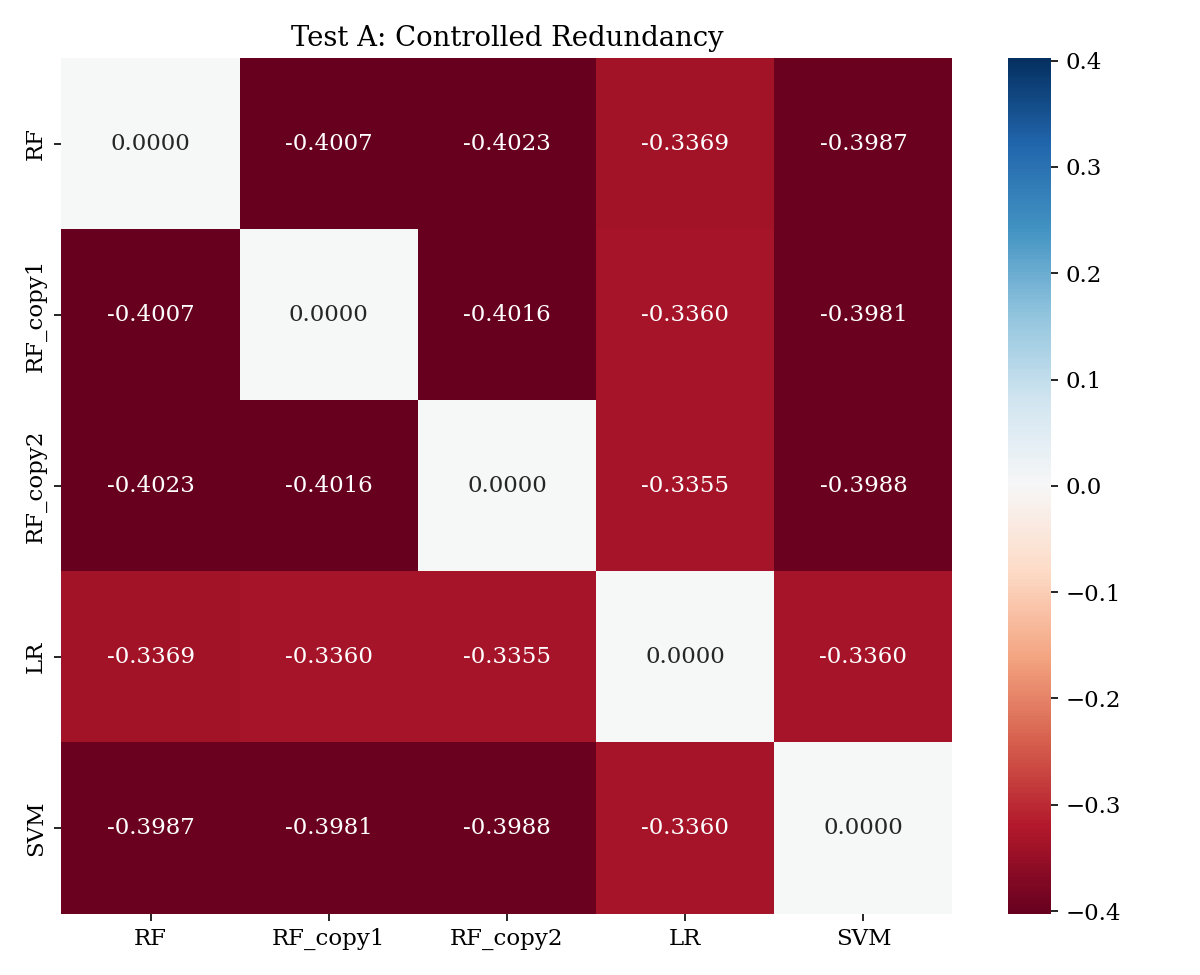
\includegraphics[width=0.85\textwidth]{fig5_test_a_heatmap}
\caption{Pairwise dividends for the controlled redundancy test. Darker red indicates stronger redundancy. The upper-left $3 \times 3$ block (RF and its two copies) is consistently darker than the cells involving LR and SVM, showing that the framework correctly identifies the artificial copies as more redundant. All values are negative because strong classifiers on tabular data produce universally negative dividends even across algorithm families; the \emph{relative} darkness is the diagnostic signal.}
\label{fig:test_a_heatmap}
\end{figure}

\subsubsection{Test B: Agreement with Established Measures}

To confirm that pairwise dividends are not measuring something idiosyncratic, they were compared against three established interaction measures: the Shapley Interaction Index (SII), which averages interactions across all possible coalition backgrounds; the Q-statistic, a classical measure of classifier agreement \citep{kuncheva2003measures}; and the disagreement measure, the fraction of instances where two models disagree.

The pairwise dividends correlated with the SII at $r = 0.964$, with the Q-statistic at $r = -0.855$, and with the disagreement measure at $r = 0.815$. The near-perfect agreement with the SII is particularly important: it means the simpler Harsanyi-based measure, which evaluates interactions with no other models present, gives essentially the same answer as the more expensive coalition-averaged measure, at least for a five-model pool. No model pairs showed contradictory signals between the two measures.

Figure~\ref{fig:dividend_heatmap} shows the full pairwise dividend matrix for the heterogeneous five-model pool. Every pair is negative, meaning all five models overlap to some degree. The most redundant pair is SVM--XGB ($-0.351$), and the least redundant is KNN--LR ($-0.249$). \textbf{Test B passed.}

\begin{figure}[htbp]
\centering
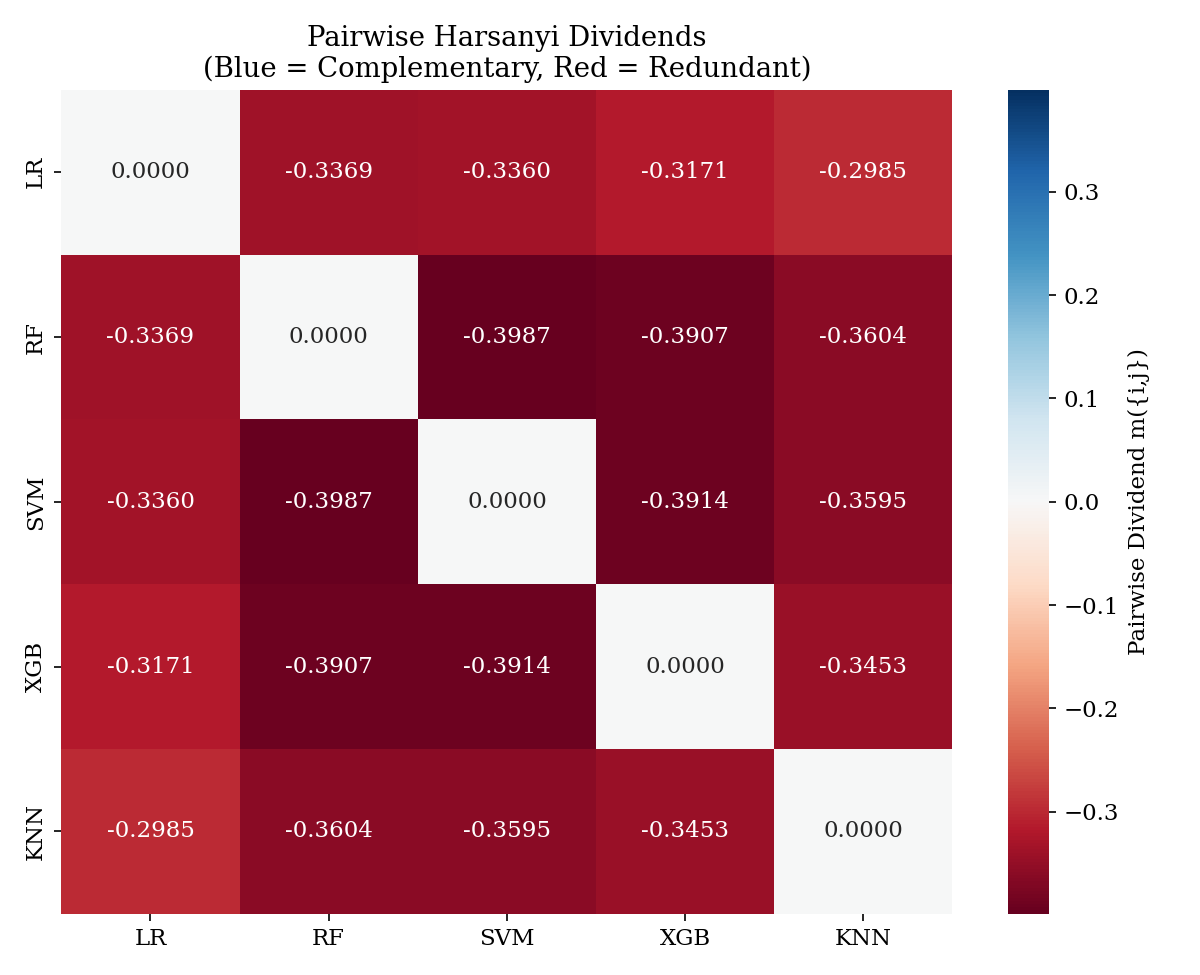
\includegraphics[width=0.85\textwidth]{fig1_dividend_heatmap}
\caption{Pairwise dividend matrix for the five base models used in the study. Red cells indicate redundancy (overlapping predictions); blue would indicate complementarity (models filling each other's gaps). All pairs are redundant, but to different degrees: SVM--XGB is the most redundant pair ($-0.351$), while KNN--LR is the least ($-0.249$).}
\label{fig:dividend_heatmap}
\end{figure}

\subsubsection{Test C: Smooth Response to Increasing Similarity}

To verify that dividends change gradually rather than erratically, a blended model was created that smoothly transitions from pure Logistic Regression (at $\alpha = 0$) to a pure copy of Random Forest (at $\alpha = 1$). At each step, the pairwise dividend between the blended model and RF was measured.

As shown in Figure~\ref{fig:test_c_monotonicity}, the dividend decreased monotonically as the blended model became more similar to RF, with a Spearman correlation of $r = -0.991$. This confirms that dividends respond continuously and predictably to increasing similarity and do not jump erratically or miss gradual changes. \textbf{Test C passed.}

\begin{figure}[htbp]
\centering
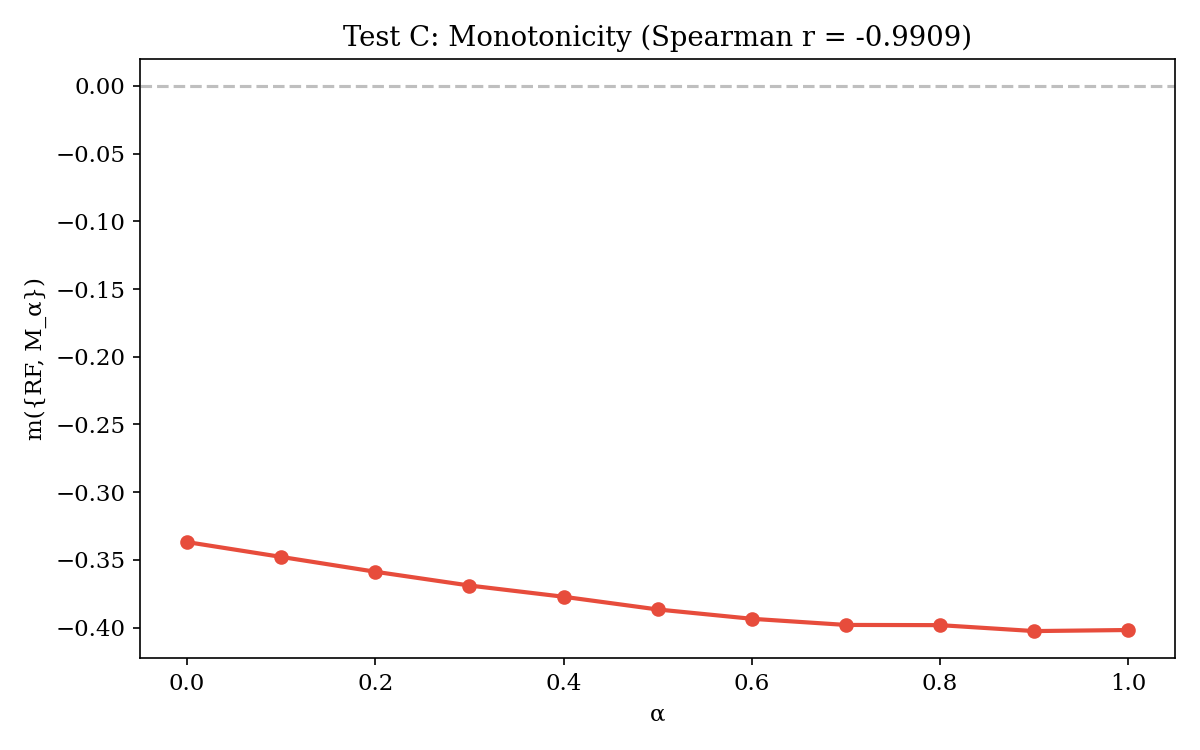
\includegraphics[width=0.75\textwidth]{fig6_test_c_monotonicity}
\caption{Pairwise dividend as a function of the blending coefficient $\alpha$. At $\alpha = 0$, the blended model is pure LR (different from RF), and the dividend is at its least negative value ($-0.265$). As $\alpha$ increases toward 1, the blended model becomes a copy of RF, and the dividend drops steadily to $-0.333$. The smooth, monotonic decline (Spearman $r = -0.991$) confirms that pairwise dividends track model similarity in a continuous and predictable manner.}
\label{fig:test_c_monotonicity}
\end{figure}

\subsubsection{Test D: Negative Control with Independent Models}

This test trained five models on completely separate feature subsets, so their errors should be independent. However, the test used accuracy instead of AUC-ROC as the performance metric, which changed the measurement scale: accuracy ranges from 0 to 1, while AUC-ROC ranges from 0.5 to 1. This shift inflated the dividend magnitudes, making it impossible to fairly compare against Tests A--C. \textbf{Test D was inconclusive} due to this measurement scale mismatch, which is acknowledged as a design limitation. Future work should replicate Test D using AUC-ROC as the performance metric throughout to ensure comparable scales.

\subsubsection{Construct Validity Summary}

Three of four tests passed convincingly. Pairwise dividends reliably detect redundancy (Test A), agree with established interaction measures (Test B), and respond smoothly to changing model similarity (Test C). The negative control (Test D) was inconclusive due to a measurement scale design error, not a failure of the dividends themselves. Overall, the construct validity of pairwise dividends as measures of model interaction is \textbf{partially supported}.

\subsection{Diagnostic Checks}

Before examining the main experiments, three diagnostic checks assessed whether the mathematical assumptions underlying the framework held in practice across all fifteen benchmark datasets and five random seeds.

\subsubsection{Decomposition Coverage}

The methodology defined decomposition coverage as the fraction of the total ensemble value explained by singleton and pairwise terms, with the expectation that it would be close to 100\%. In practice, coverage was strongly negative across all fifteen datasets, ranging from $-2.58$ to $-4.98$ (Figure~\ref{fig:diagnostics}, left panel).

This outcome does not indicate a failure of the framework. Each model individually contributes a positive singleton dividend (around $+0.35$), and there are five of them ($\approx +1.75$ total). But each pair of models produces a negative pairwise dividend (around $-0.30$), and there are ten such pairs ($\approx -3.00$ total). The sum is roughly $-1.25$, while the actual ensemble improvement over random guessing is only about $+0.40$. The mismatch confirms that higher-order terms (three-way and above) are large and positive, compensating for the pervasive pairwise redundancy. The practical implication is that this metric should be read as a redundancy diagnostic rather than a completeness measure.

\subsubsection{Monotonicity Violations and Grand Coalition Performance}

The monotonicity violation rate ranged from 2.7\% to 47.8\% across datasets (Figure~\ref{fig:diagnostics}, center panel). Six datasets exceeded the 40\% threshold on at least one random seed, and no single model was consistently the culprit. Relatedly, the full five-model ensemble was the best-performing coalition in only 6 of 75 runs (8\%). In the remaining 69 runs, some smaller subset outperformed the full pool. This is a natural consequence of model redundancy, as averaging five partially overlapping models can be worse than combining just the most distinct subset.

\subsubsection{Rank Stability}

The rank-stability check verified whether the relative ordering of models changes when coalition values are recomputed using coopetitive weights instead of equal weights. The Spearman correlation was 1.0 in all 75 runs (Figure~\ref{fig:diagnostics}, right panel), confirming that model rankings are preserved under the framework's weighting scheme. However, with only $n = 5$ models the number of distinct possible rankings is small, and perfect rank preservation across all seeds provides limited diagnostic value; a larger pool would be needed for this check to be informative.

\begin{figure}[htbp]
\centering
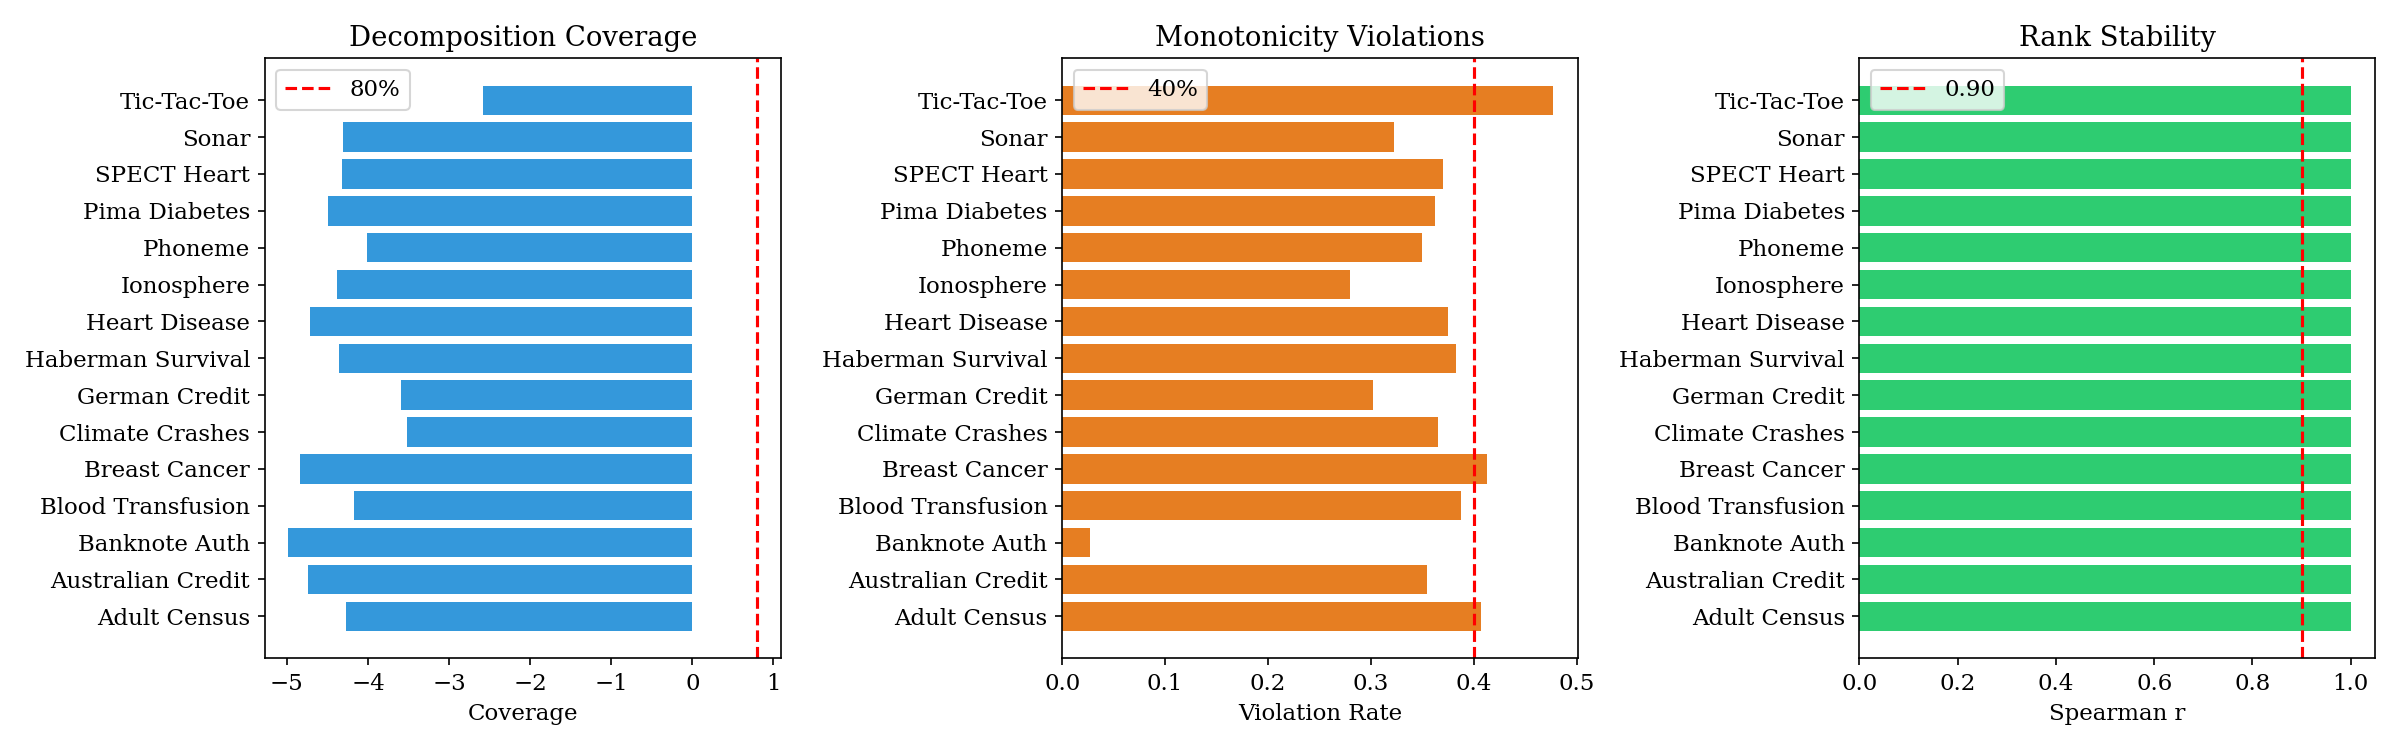
\includegraphics[width=\textwidth]{fig7_diagnostics}
\caption{Three diagnostic checks across all 15 datasets (averaged over 5 seeds). \textbf{Left:} Decomposition coverage is universally negative because pairwise redundancy terms outweigh singleton contributions; the 80\% threshold (red dashed line) is never met. \textbf{Center:} Monotonicity violation rates mostly fall between 20\% and 45\%, indicating that adding a model sometimes reduces coalition performance. \textbf{Right:} Rank stability (Spearman $r$) is uniformly 1.0 across all runs and seeds.}
\label{fig:diagnostics}
\end{figure}

\subsection{Experiment 2: Ablation Study}

This experiment compared ten weighting strategies to isolate which components of the framework contribute to performance. The study trained five heterogeneous base models (LR, RF, SVM, XGB, KNN) on each of fifteen benchmark datasets with five random seeds (75 total runs per method), measuring AUC-ROC as the primary metric and negative Brier score as the secondary metric. Table~\ref{tab:ablation} shows the results averaged across all 15 datasets and 5 seeds, and Figure~\ref{fig:ablation} breaks them down per dataset.

\begin{table}[htbp]
\centering
\caption{Performance of all weighting variants, averaged across 15 datasets and 5 seeds. AUC-ROC measures discrimination (higher is better). Negative Brier score measures calibration quality; values closer to zero indicate better-calibrated predictions.}
\label{tab:ablation}
\begin{tabular}{lrr}
\toprule
\textbf{Variant} & \textbf{AUC-ROC} & \textbf{Neg.\ Brier} \\
\midrule
Coopetitive ($\lambda = 0.5$) & 0.8977 & $-0.0966$ \\
Coopetitive (CV $\lambda$) & 0.8974 & $-0.0976$ \\
Shapley & 0.8968 & $-0.0987$ \\
Performance-Weighted & 0.8958 & $-0.0999$ \\
Individual-Only ($\lambda = 0$) & 0.8958 & $-0.0999$ \\
Equal & 0.8938 & $-0.1019$ \\
Best Single Model & 0.8901 & $-0.0993$ \\
Shapley + SII & 0.8879 & $-0.1081$ \\
Stacking & 0.8852 & $-0.1117$ \\
Interaction-Only & 0.8707 & $-0.1186$ \\
\bottomrule
\end{tabular}
\end{table}

Four key patterns emerge. First, Individual-Only ($\lambda = 0$) and Performance-Weighted produce identical results (AUC $= 0.8958$), confirming the predicted algebraic equivalence: when the interaction term is turned off, the framework reduces exactly to performance-based weighting. Second, Coopetitive-0.5 (AUC $= 0.8977$) outperforms Individual-Only by $+0.0019$ and achieves the best calibration of any method (Neg.\ Brier $= -0.0966$), winning on 9 of 15 datasets. Third, Interaction-Only performed worst of all methods (AUC $= 0.8707$), confirming that effective weighting requires both individual model quality and interaction structure. Fourth, Shapley~+~SII (AUC $= 0.8879$) performed worse than plain Shapley (AUC $= 0.8968$), providing empirical evidence of the double-counting problem described in Chapter~1.

The slightly higher AUC of Coopetitive-0.5 (0.8977) relative to Coopetitive-CV (0.8974) is not paradoxical: fixed $\lambda = 0.5$ happens to be near-optimal for the datasets where marginal gains are largest, while the inner cross-validation incurs a small optimization cost by overfitting to the small validation sets used for $\lambda$ selection. This result is consistent with the H4 finding that robustness ratios average only 0.08, indicating that no single fixed $\lambda$ reliably dominates across datasets.

\begin{figure}[htbp]
\centering
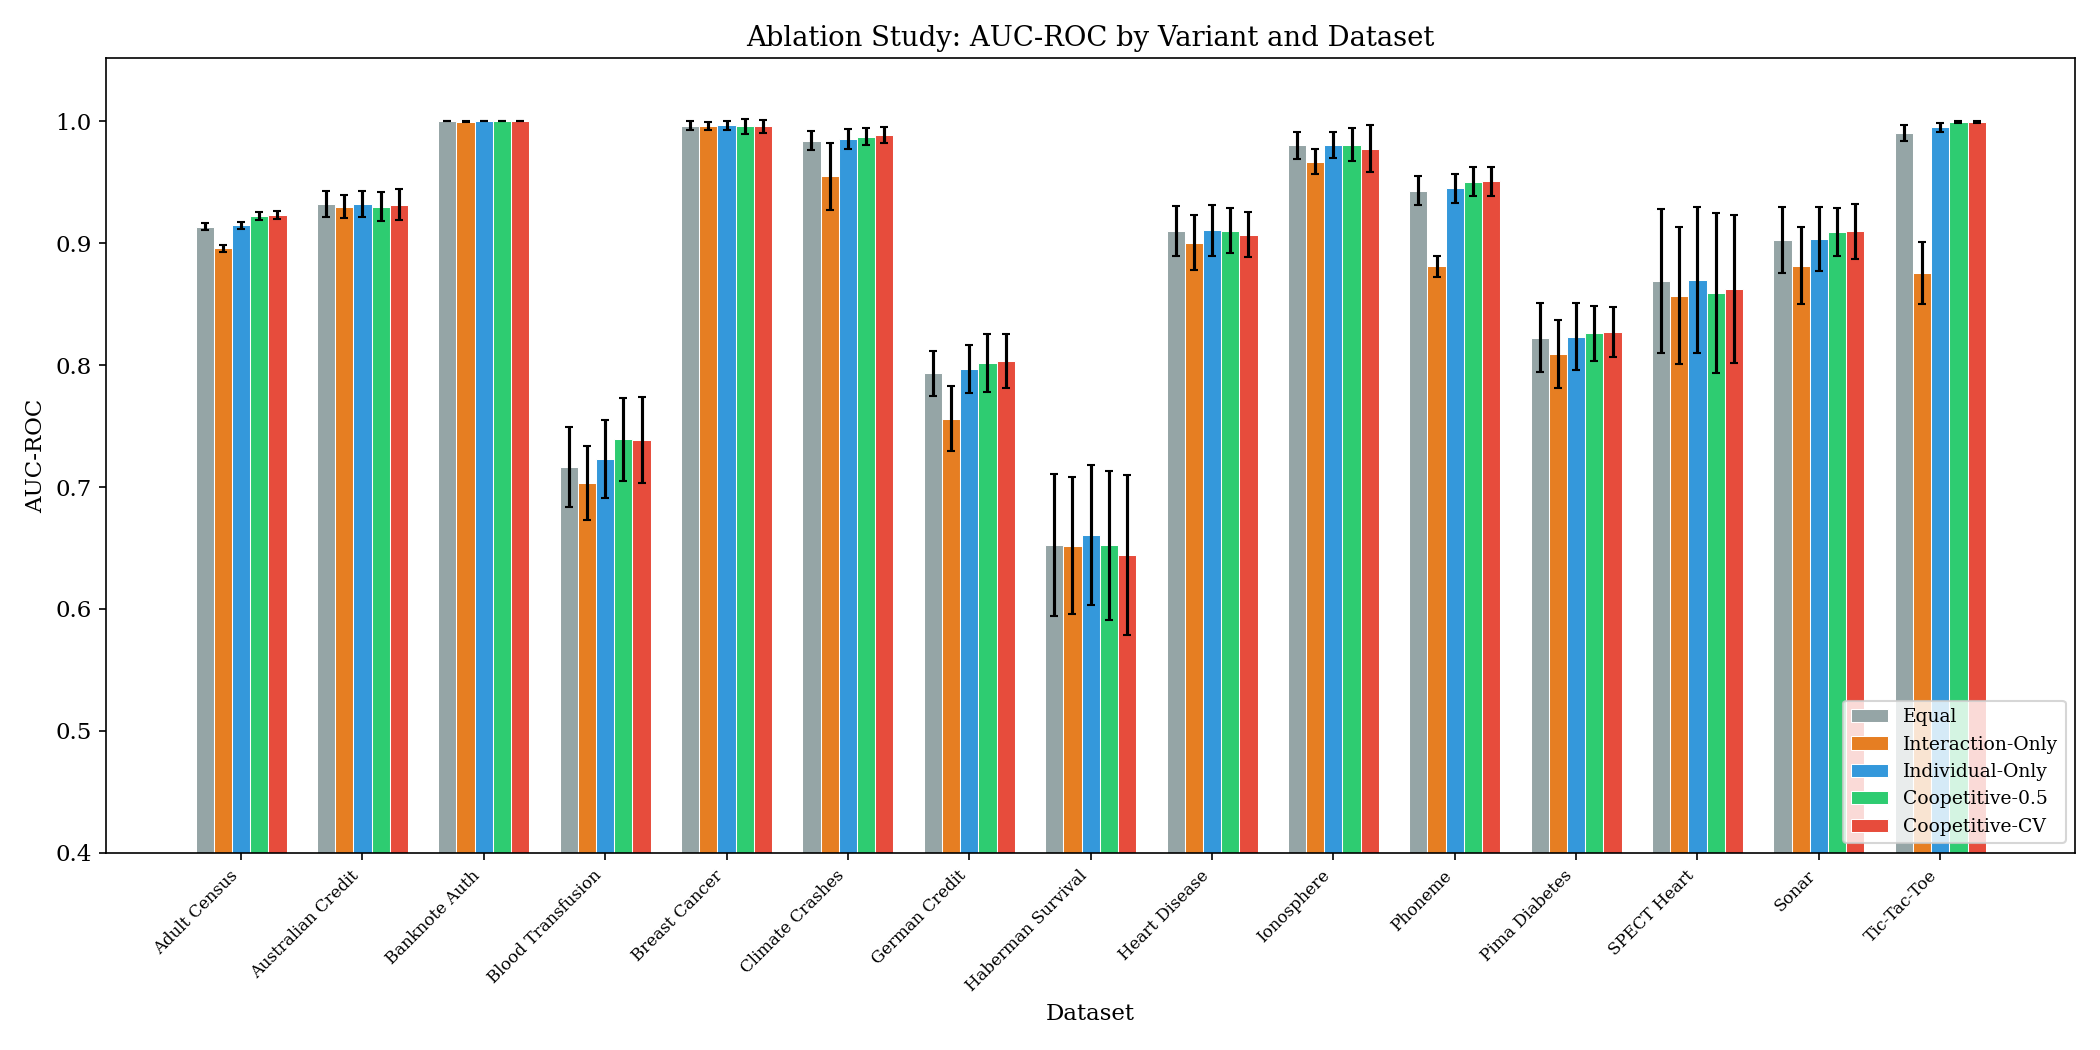
\includegraphics[width=\textwidth]{fig2_ablation_chart}
\caption{Per-dataset AUC-ROC for the five primary ablation variants. Error bars show $\pm 1$ standard deviation across five random seeds. The coopetitive variants (green and red) match or slightly exceed the Individual-Only baseline (blue) on most datasets. The Interaction-Only variant (orange) consistently underperforms across datasets.}
\label{fig:ablation}
\end{figure}

The formal statistical test for H1, a one-tailed Wilcoxon signed-rank test comparing Coopetitive-0.5 against Individual-Only across all 15 datasets, yielded $p = 0.148$, not reaching the conventional significance threshold of $p < 0.05$. The coopetitive variant won on 9 of 15 datasets, with a mean improvement of $+0.0018$ AUC and an effect size of $r = 0.294$ (small-to-medium). The non-significance is unsurprising given the very small effect size and the total AUC spread of 0.027 across all ablation variants (Table~\ref{tab:ablation}); a larger and more redundant model pool would provide a harder test of H1. At the same time, the alternative interpretation cannot be dismissed: the null hypothesis may be correct and the interaction term may genuinely add no value beyond performance-weighted ensembling in standard heterogeneous pools on tabular data. \textbf{H1 is not statistically supported, but the direction of the evidence is consistent with the hypothesis.}

\subsection{Experiment 3: Benchmark Comparison}

The coopetitive framework was benchmarked against five established ensemble strategies. Following the nonparametric multi-dataset comparison methodology of \citet{demsar2006statistical}, performance was assessed using Friedman test rankings, where a lower average rank indicates the method won more often across datasets. Table~\ref{tab:benchmark} shows the results, and Figure~\ref{fig:benchmark_ranks} visualizes the ranking ordering.

\begin{table}[htbp]
\centering
\caption{Benchmark comparison: methods ranked by how often they outperformed others across 15 datasets (lower rank is better). Mean AUC-ROC is also shown for reference.}
\label{tab:benchmark}
\begin{tabular}{lrr}
\toprule
\textbf{Method} & \textbf{Avg.\ Rank} & \textbf{Mean AUC} \\
\midrule
Shapley & 2.80 & 0.8968 \\
Coopetitive-CV & 2.87 & 0.8974 \\
Performance-Weighted & 3.23 & 0.8958 \\
Stacking & 3.50 & 0.8852 \\
Best Single Model & 4.20 & 0.8901 \\
Equal & 4.40 & 0.8938 \\
\bottomrule
\end{tabular}
\end{table}

Note that the ablation (Table~\ref{tab:ablation}) and benchmark (Table~\ref{tab:benchmark}) experiments use partially overlapping but distinct method sets; Coopetitive-0.5, which leads on mean AUC in the ablation, is not included in the benchmark ranking, and Friedman average rank can diverge from mean AUC when the performance distribution across datasets is skewed. Coopetitive-CV and Shapley occupied the top two positions in the benchmark with nearly identical average ranks (2.87 vs.\ 2.80). Both game-theoretic methods clearly outranked Stacking (3.50), Best Single Model (4.20), and Equal weighting (4.40). On the secondary calibration metric, Coopetitive-0.5 achieved the best negative Brier score ($-0.097$) of any method, ahead of Shapley ($-0.099$) and Stacking ($-0.112$).

The Friedman test yielded $p = 0.072$, which is suggestive of real differences between methods but not significant at $p < 0.05$. \textbf{H3 is not statistically supported, but the coopetitive framework achieves a competitive ranking and the best probability calibration of all methods tested.}

\begin{figure}[htbp]
\centering
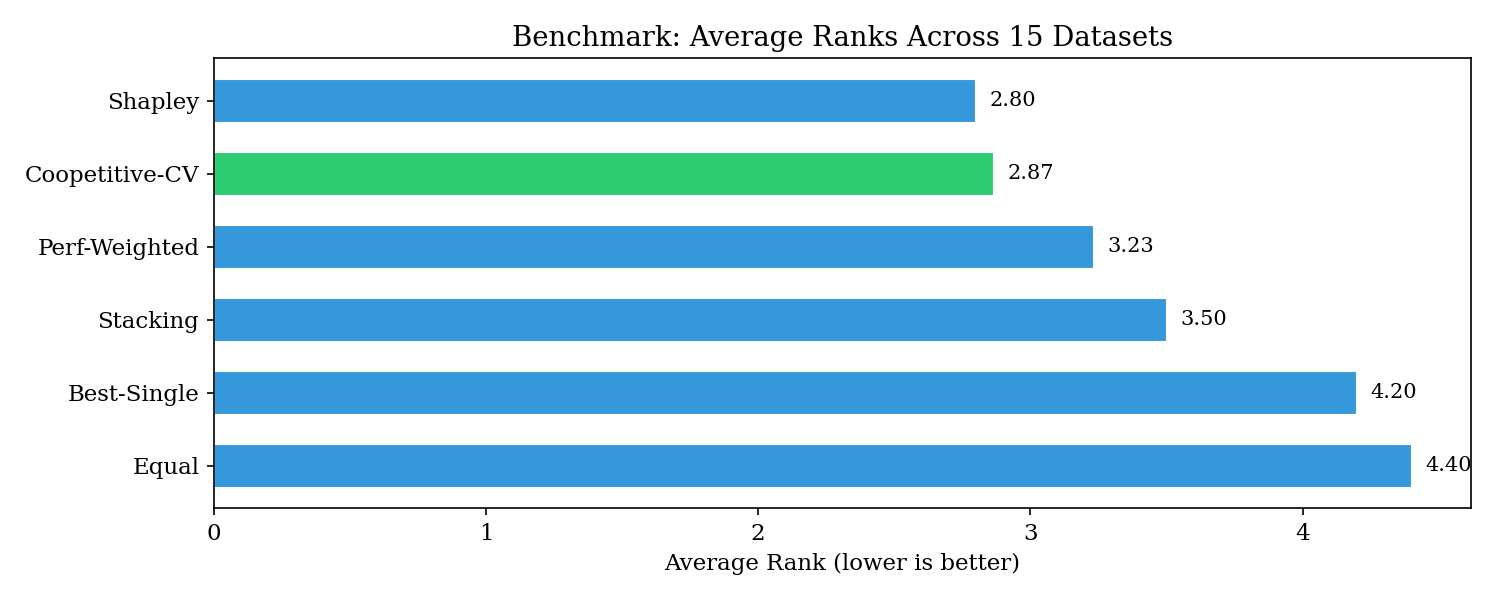
\includegraphics[width=0.85\textwidth]{fig3_critical_difference}
\caption{Average rankings across 15 datasets (lower is better). Shapley and Coopetitive-CV are nearly tied at the top, both clearly ahead of Stacking, Best Single Model, and Equal weighting. The Friedman test ($p = 0.072$) suggests meaningful differences but does not reach $p < 0.05$.}
\label{fig:benchmark_ranks}
\end{figure}

\subsection{Experiment 4: Lambda Sensitivity}

This experiment characterized how sensitive ensemble performance is to the $\lambda$ parameter, which controls the trade-off between individual model quality and interaction structure. A sweep of $\lambda \in [0, 2.0]$ in steps of 0.1 was conducted across all fifteen datasets, with performance measured by AUC-ROC at each value. At $\lambda = 0$, the framework ignores interactions entirely and reduces to performance-weighted ensembling; as $\lambda$ increases, the complementarity and redundancy structure of the pool exerts more influence on the final weights.

Table~\ref{tab:lambda} and Figure~\ref{fig:lambda_sensitivity} show the optimal $\lambda$ for each dataset. There is no single best value: the optimal $\lambda$ ranged from 0.0 (Banknote Authentication, Sonar) to 1.5 (Australian Credit), with a mean of $0.67 \pm 0.45$.

\begin{table}[htbp]
\centering
\caption{Optimal $\lambda$ for each dataset. The wide range (0.0 to 1.5) shows that no fixed default works well everywhere.}
\label{tab:lambda}
\begin{tabular}{lrr}
\toprule
\textbf{Dataset} & $\boldsymbol{\lambda^*}$ & \textbf{AUC at $\lambda^*$} \\
\midrule
Adult Census & 0.8 & 0.9233 \\
Australian Credit & 1.5 & 0.9318 \\
Banknote Auth.\ & 0.0 & 1.0000 \\
Blood Transfusion & 1.3 & 0.7449 \\
Breast Cancer & 1.0 & 0.9972 \\
Climate Crashes & 0.7 & 0.9883 \\
German Credit & 0.1 & 0.8029 \\
Haberman Survival & 0.6 & 0.6532 \\
Heart Disease & 0.3 & 0.9106 \\
Ionosphere & 0.4 & 0.9822 \\
Phoneme & 0.7 & 0.9512 \\
Pima Diabetes & 0.9 & 0.8267 \\
SPECT Heart & 1.1 & 0.8729 \\
Sonar & 0.0 & 0.9109 \\
Tic-Tac-Toe & 0.7 & 0.9999 \\
\bottomrule
\end{tabular}
\end{table}

Figure~\ref{fig:lambda_sensitivity} reveals three distinct patterns by dataset difficulty. For easy datasets where all models already perform near-perfectly (Banknote Authentication, Breast Cancer), performance is flat across all $\lambda$ values because the interaction terms are negligibly small. For moderately difficult datasets (Adult Census, Climate Crashes, Phoneme), performance peaks around $\lambda = 0.5$--$0.8$ then declines. For the most difficult datasets (Blood Transfusion, Haberman Survival), larger $\lambda$ values (1.0--1.5) work best, suggesting that these datasets benefit most from aggressively downweighting redundant models.

The proposed fixed default of $\lambda = 0.5$ achieved 95\% of optimal performance on only 13\% of datasets, and the robustness ratio averaged just 0.08. To be precise: a robustness ratio of 0.08 means that fewer than two of the twenty-one grid points in $\lambda \in [0, 2.0]$ fall within 95\% of the dataset-specific optimum on average. It is not a raw-performance ratio---$\lambda = 0.5$ does not achieve only 8\% of optimal AUC---but rather a measure of how narrowly concentrated the near-optimal region of the parameter space is, and how rarely $\lambda = 0.5$ happens to land in that region. A repeated-measures ANOVA confirmed that $\lambda$ sensitivity is dataset-dependent ($F = 7.28$, $p_{\text{GG}} = 0.013$, Greenhouse--Geisser corrected due to violated sphericity). \textbf{H4 is not supported.} There is no universal fixed $\lambda$; cross-validated selection (Coopetitive-CV) is the recommended deployment strategy.

\begin{figure}[htbp]
\centering
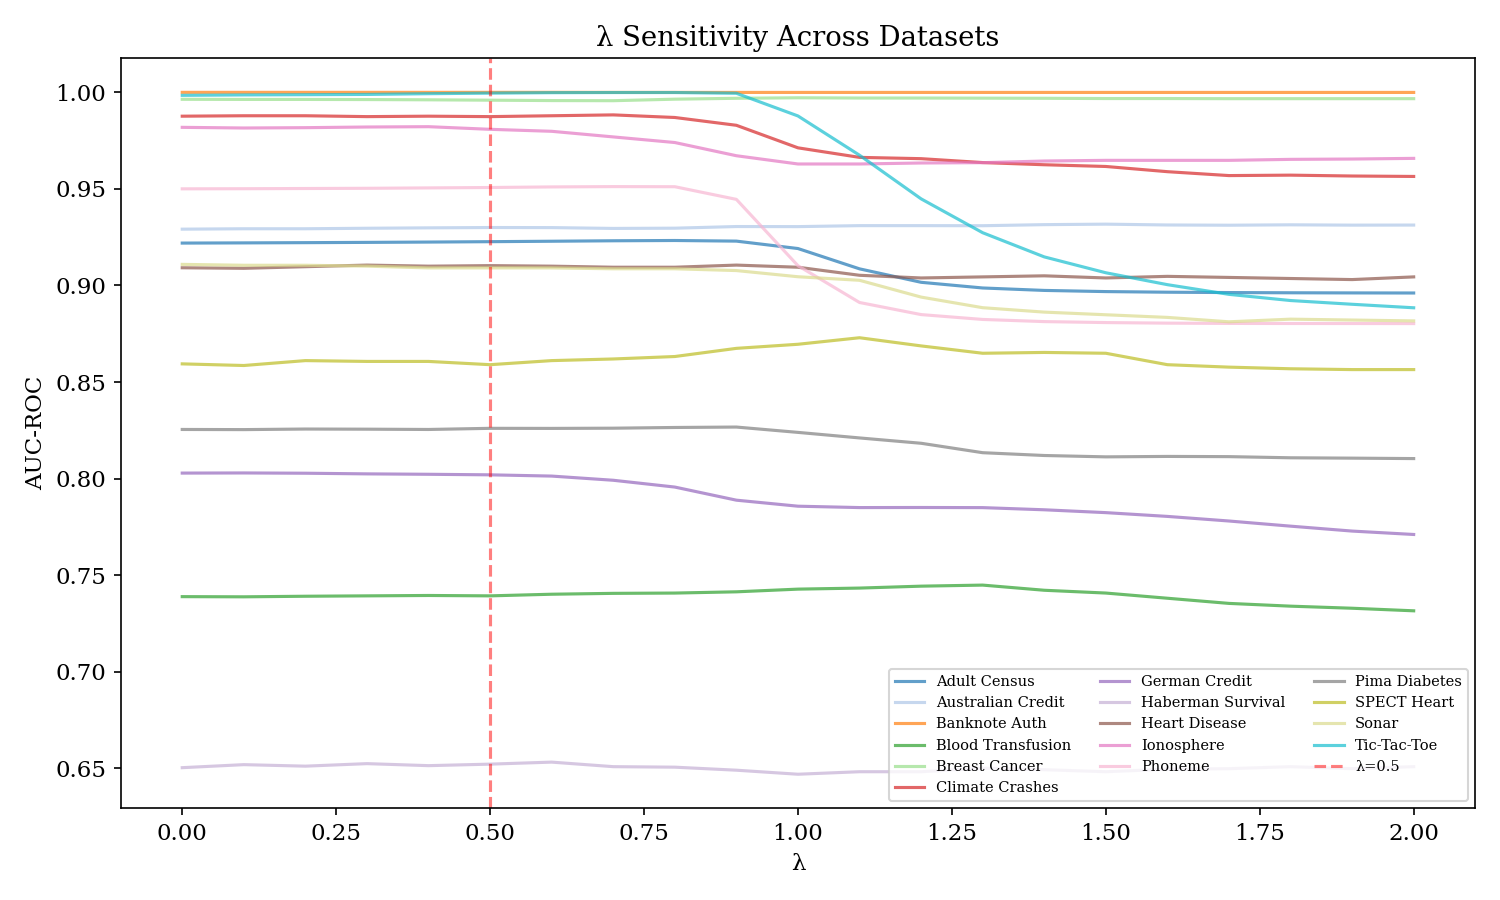
\includegraphics[width=\textwidth]{fig4_lambda_sensitivity}
\caption{AUC-ROC as a function of $\lambda$ for all 15 datasets. The red dashed line marks the proposed default $\lambda = 0.5$. Easy datasets (top, near 1.0) are flat, as $\lambda$ does not matter when all models are already excellent. Moderate datasets (middle) peak around $\lambda = 0.5$--$0.8$. Difficult datasets (bottom) are more variable and often prefer larger $\lambda$. The non-parallel curves confirm that the optimal $\lambda$ is dataset-dependent, ruling out a universal fixed default.}
\label{fig:lambda_sensitivity}
\end{figure}

\subsection{Hypothesis Summary}

Table~\ref{tab:hypotheses} summarizes the outcome of all four hypotheses tested in this study.

\begin{table}[htbp]
\centering
\caption{Summary of hypothesis testing results.}
\label{tab:hypotheses}
\begin{tabular}{p{3.6cm}p{3.2cm}p{5.5cm}}
\toprule
\textbf{Hypothesis} & \textbf{Result} & \textbf{Key Evidence} \\
\midrule
H1: Adding interaction information improves performance & Not significant ($p = 0.148$) & Wins on 9/15 datasets, $+0.0018$ mean AUC, best Brier score \\
H2: Dividends accurately detect model relationships & Partially supported & 3/4 controlled tests pass; negative control inconclusive due to design error \\
H3: Framework is competitive with standard methods & Not significant ($p = 0.072$) & Ranks 2nd of 6 methods; best calibration \\
H4: A fixed $\lambda = 0.5$ works well everywhere & Not supported & Optimal $\lambda$ ranges from 0.0 to 1.5; cross-validation needed \\
\bottomrule
\end{tabular}
\end{table}

\section{Discussion}

This section interprets the patterns in the results reported in Section~4.1, explaining the mechanisms behind each finding and their implications for ensemble learning practice. Figures are not repeated here; the reader is referred to the relevant subsections in Section~4.1.

\subsection{Interpretable Diagnostics as the Primary Contribution}

The pairwise dividend matrix offers something that no other ensemble method provides: a pairwise, interpretable map of which models overlap and which are most distinct. From the matrix, a practitioner can immediately identify the most redundant pair and the least redundant pair in the pool. If budget constraints require dropping a model, the matrix directly identifies candidates whose removal would incur the least loss of complementarity. If a new model is being considered for the pool, its pairwise dividends with existing members immediately reveal whether it adds genuine diversity or merely more redundancy. Stacking, equal weighting, and performance-proportional weighting offer no comparable diagnostic capability.

This interpretability benefit is independent of whether the coopetitive weights themselves improve upon simpler baselines, and it constitutes the framework's most durable practical contribution. The diagnostic value is also directly applicable to automated machine learning pipelines, ensemble pruning tools, and any setting where interpretable model relationship information is valued alongside raw predictive accuracy. The quantitative performance results reported in \S\S\,4.1.3--4.1.4 should be read as secondary evidence: they characterize the magnitude of any performance trade-off relative to simpler baselines, not the primary reason to adopt the framework.

However, the results also reveal an important limitation of the ``coopetitive'' framing. In theory, the framework encompasses both a cooperative regime---where positive dividends indicate complementarity---and a competitive regime---where negative dividends indicate redundancy. In practice, all pairwise dividends across all fifteen datasets were negative, meaning the cooperative half of the coopetitive duality never appeared in this study's setting. Positive dividends would more likely arise from weaker or more diverse base models (e.g., models trained on different feature subsets or data modalities), from small or noisy datasets where different models make genuinely different errors, or from settings where some models are deliberately weak. In the present setting---five well-optimized classifiers on standard tabular binary-classification benchmarks---the framework functioned entirely as a redundancy-penalty mechanism. The term ``coopetitive'' remains aspirationally apt, describing the potential dual character of the formula, but practitioners should be aware that in well-optimized heterogeneous pools the competitive component will dominate.

\subsection{Role of the Interaction Term}

The interaction term in the coopetitive formula functions primarily as a redundancy penalty. Because nearly all pairwise dividends are negative across all datasets, increasing $\lambda$ effectively downweights models that overlap heavily with many others and upweights models that are more distinct from the pool. The performance improvement is modest ($+0.0018$ AUC) because the five heterogeneous models in the pool are already reasonably diverse, leaving the interaction term limited room to improve an arrangement that is already decent. In pools with greater redundancy, such as multiple gradient boosting variants with different hyperparameter settings, the penalty mechanism would exert a stronger effect, and the gain over simpler baselines could be correspondingly larger. The modest gain observed here should therefore not be interpreted as evidence that the interaction term is unimportant in general, but rather as a consequence of the specific diversity level of the five-model heterogeneous pool used in this study.

\subsection{Empirical Confirmation of the Double-Counting Problem}

One of the clearest findings is that the Shapley~+~SII variant performed worse than plain Shapley by 0.009 AUC. This is the empirical confirmation of the double-counting problem motivating the entire framework: when interaction effects already embedded within the Shapley value are added again through the Shapley Interaction Index, the resulting weights are distorted and performance drops. The M\"{o}bius-based framework avoids this by construction, since singleton and pairwise dividends are mathematically non-overlapping. The magnitude of this degradation (0.009 AUC) is meaningful given that the total AUC spread across the ten ablation variants (Table~\ref{tab:ablation}) is only 0.027, meaning the double-counting cost represents roughly one-third of the available performance range between the best and worst weighting strategies in the study.

\subsection{Why Stacking Underperformed}

Stacking is typically considered a strong baseline \citep{wolpert1992stacking}, but it ranked fourth here (rank 3.50, AUC $= 0.8852$). The most plausible explanation is sample size. Eleven of the fifteen benchmark datasets have fewer than 1,000 samples, and the 20\% validation split gives the meta-learner as few as 40--60 training instances. With five correlated base model predictions as input features and only a few dozen rows to learn from, the logistic regression meta-learner is likely to overfit---a well-known risk when the number of training instances is small relative to the number of input features. Game-theoretic methods sidestep this problem entirely because they derive weights from the combinatorial structure of 32 coalition values, which does not require fitting parameters to small samples. In larger-sample settings, we conjecture that stacking would perform better or potentially surpass the game-theoretic methods, as the meta-learner would have sufficient data to learn meaningful combination weights.

\subsection{The Decomposition Coverage Issue}

The universally negative coverage values ($-2.6$ to $-5.0$) are a direct consequence of truncating the M\"{o}bius decomposition to only two orders. In a pool of five strong, partially overlapping classifiers, the ten pairwise redundancy terms overwhelm the five positive singleton terms. The missing higher-order terms (10 three-way, 5 four-way, and 1 five-way interaction) would restore the balance, but computing and interpreting them is beyond the scope of this study. The practical takeaway is that this metric should not be read as a completeness measure but as a diagnostic flag: strongly negative values indicate a pool dominated by pairwise redundancy, signaling that the pool would benefit from either a more diverse model selection or explicit higher-order interaction terms in the weighting formula.

\subsection{Why \texorpdfstring{$\lambda$}{lambda} Cannot Be Fixed}

The optimal $\lambda$ varies from 0.0 (for easy datasets where interaction reweighting adds only noise) to 1.5 (for difficult datasets where aggressive redundancy penalization helps). This makes intuitive sense: when every model in the pool already achieves near-perfect accuracy, there is very little redundancy to penalize, and adjusting weights based on interaction structure introduces noise rather than signal. When models struggle and overlap substantially in their errors, a larger $\lambda$ more forcefully redirects weight toward the most distinct models, yielding a more robust ensemble. The practical consequence is that the framework should always be deployed with cross-validated $\lambda$ selection. This adds almost no computational cost because the inner cross-validation operates on cached probability predictions and no models need to be retrained.

\subsection{Grand Coalition Is Not Always Best}

In 92\% of experimental runs, some subset of models outperformed the full five-model ensemble. This is not a flaw in the framework but a reflection of the redundancy in the pool: averaging five partially overlapping models can be worse than combining just the three or four most distinct ones. The dividend matrix provides exactly the information needed to identify which models to retain and which to exclude, suggesting that future work should combine the coopetitive weighting mechanism with a dividend-informed pruning step to further improve performance by first excluding the most redundant models before applying ensemble combination.

% ============================================================
% CHAPTER 5: CONCLUSION
% ============================================================
\chapter{Conclusion}

The most durable contribution of this study is the pairwise dividend matrix: an interpretable diagnostic map of pairwise model redundancy that no other ensemble method provides. From this matrix, practitioners can immediately identify the most redundant pair in the pool, rank candidate models for removal by their redundancy cost, and assess whether a new model adds genuine diversity---information that stacking, equal weighting, and performance-proportional approaches do not offer. This diagnostic capability is independent of the quantitative performance results and is directly applicable to automated machine learning pipelines, ensemble pruning tools, and any setting where interpretable model relationship information is valued alongside raw predictive accuracy. It is grounded in the M\"{o}bius decomposition of the characteristic function, which uniquely separates individual model quality from pairwise interaction effects without double-counting.

On quantitative performance, the most unambiguous finding is the empirical confirmation of double-counting: the Shapley~+~SII variant degraded performance by 0.009 AUC relative to plain Shapley, representing roughly one-third of the total performance spread across all ablation variants. Construct validity was partially established: three of four controlled tests confirmed that pairwise dividends correctly detect redundancy, agree with established interaction measures ($r = 0.964$ with the SII), and respond smoothly to changing model similarity. Test D was inconclusive not because the dividends failed to detect independence, but because a measurement design error---using accuracy instead of AUC-ROC, which altered the numeric scale---made the results uninterpretable; future work should replicate this test with a consistent metric. In the benchmark comparison, Coopetitive-CV ranked second among six methods and achieved the best probability calibration of all methods tested (Neg.\ Brier $= -0.097$).

Several limitations constrain these findings. The decomposition is truncated to singleton and pairwise terms, omitting higher-order interactions that the strongly negative coverage values suggest are substantial. Pairwise dividends evaluate interactions at the empty coalition only, so the observed agreement with the SII may not hold for larger or more heterogeneous pools. The study is confined to binary classification, and exact coalition evaluation scales exponentially, limiting the framework to pools of $n \leq 12$ without approximation. The rank-stability check showed perfect Spearman correlation across all runs, but with only $n = 5$ models this result is uninformative---a larger pool is needed to meaningfully test this property. The optimal $\lambda$ varied widely across datasets (0.0 to 1.5), ruling out a universal fixed default and requiring cross-validated selection for deployment. The most direct extensions are higher-order dividends (three-way and above), which this study truncates for parsimony but which the strongly negative coverage values suggest are substantial, and larger model pools, which would also provide a more informative rank-stability diagnostic. Multi-class classification and regression settings are natural further boundaries to test. Online and streaming scenarios represent a longer-term direction and would establish whether the interpretable diagnostic value demonstrated here for offline evaluation translates to real-time ensemble management in production systems.

% ============================================================
% BIBLIOGRAPHY
% ============================================================
\bibliographystyle{apalike}

\begin{thebibliography}{99}

\bibitem[Bimonte et~al., 2024]{bimonte2024mortality}
Bimonte, G., Russolillo, M., Shang, H.~L., \& Yang, Y. (2024).
\newblock Mortality models ensemble via Shapley value.
\newblock {\em Decisions in Economics and Finance}.
\newblock \url{https://doi.org/10.1007/s10203-024-00455-z}

\bibitem[Brandenburger \& Nalebuff, 1996]{brandenburger1996coopetition}
Brandenburger, A.~M., \& Nalebuff, B.~J. (1996).
\newblock {\em Co-opetition}.
\newblock Doubleday.

\bibitem[Breiman, 1996]{breiman1996bagging}
Breiman, L. (1996).
\newblock Bagging predictors.
\newblock {\em Machine Learning}, 24(2), 123--140.

\bibitem[Dehez, 2017]{dehez2017harsanyi}
Dehez, P. (2017).
\newblock On Harsanyi dividends and asymmetric values.
\newblock {\em International Game Theory Review}, 19(3), 1--36.
\newblock \url{https://doi.org/10.1142/S0219198917500128}

\bibitem[Dem\v{s}ar, 2006]{demsar2006statistical}
Dem\v{s}ar, J. (2006).
\newblock Statistical comparisons of classifiers over multiple data sets.
\newblock {\em Journal of Machine Learning Research}, 7, 1--30.

\bibitem[Fawcett, 2006]{fawcett2006roc}
Fawcett, T. (2006).
\newblock An introduction to ROC analysis.
\newblock {\em Pattern Recognition Letters}, 27(8), 861--874.

\bibitem[Freund \& Schapire, 1997]{freund1997adaboost}
Freund, Y., \& Schapire, R.~E. (1997).
\newblock A decision-theoretic generalization of on-line learning and an application to boosting.
\newblock {\em Journal of Computer and System Sciences}, 55(1), 119--139.

\bibitem[Grabisch \& Roubens, 1999]{grabisch1999axiomatic}
Grabisch, M., \& Roubens, M. (1999).
\newblock An axiomatic approach to the concept of interaction among players in cooperative games.
\newblock {\em International Journal of Game Theory}, 28(4), 547--565.

\bibitem[Harsanyi, 1959]{harsanyi1959bargaining}
Harsanyi, J.~C. (1959).
\newblock A bargaining model for cooperative $n$-person games.
\newblock In A.~W. Tucker \& R.~D. Luce (Eds.), {\em Contributions to the Theory of Games IV} (pp.~325--355). Princeton University Press.

\bibitem[Harsanyi, 1963]{harsanyi1963simplified}
Harsanyi, J.~C. (1963).
\newblock A simplified bargaining model for the $n$-person cooperative game.
\newblock {\em International Economic Review}, 4(2), 194--220.

\bibitem[Margineantu \& Dietterich, 1997]{margineantu1997pruning}
Margineantu, D.~D., \& Dietterich, T.~G. (1997).
\newblock Pruning adaptive boosting.
\newblock In {\em Proceedings of the 14th International Conference on Machine Learning} (pp.~211--218).

\bibitem[Kuncheva \& Whitaker, 2003]{kuncheva2003measures}
Kuncheva, L.~I., \& Whitaker, C.~J. (2003).
\newblock Measures of diversity in classifier ensembles and their relationship with the ensemble accuracy.
\newblock {\em Machine Learning}, 51(2), 181--207.

\bibitem[Muschalik et~al., 2024]{muschalik2024shapiq}
Muschalik, M., Baniecki, H., Fumagalli, F., Kolpaczki, P., Hammer, B., \& H\"{u}llermeier, E. (2024).
\newblock shapiq: Shapley interactions for machine learning.
\newblock {\em NeurIPS 2024, Datasets and Benchmarks Track}.

\bibitem[Rozemberczki \& Sarkar, 2021]{rozemberczki2021shapley}
Rozemberczki, B., \& Sarkar, R. (2021).
\newblock The Shapley value of classifiers in ensemble games.
\newblock In {\em Proceedings of the 30th ACM International Conference on Information and Knowledge Management} (pp.~1558--1567).

\bibitem[Rozemberczki et~al., 2022]{rozemberczki2022shapley}
Rozemberczki, B., Watson, L., Bayer, P., Yang, H.-T., Kiss, O., Nilsson, S., \& Sarkar, R. (2022).
\newblock The Shapley value in machine learning.
\newblock In {\em Proceedings of IJCAI-22} (pp.~5572--5579).

\bibitem[Shapley, 1953]{shapley1953value}
Shapley, L.~S. (1953).
\newblock A value for $n$-person games.
\newblock In {\em Contributions to the Theory of Games II} (pp.~307--317). Princeton University Press.

\bibitem[Tsai et~al., 2023]{tsai2023faith}
Tsai, C.-P., Yeh, C.-K., \& Ravikumar, P. (2023).
\newblock Faith-Shap: The faithful Shapley interaction index.
\newblock {\em Journal of Machine Learning Research}, 24(94), 1--42.

\bibitem[Wolpert, 1992]{wolpert1992stacking}
Wolpert, D.~H. (1992).
\newblock Stacked generalization.
\newblock {\em Neural Networks}, 5(2), 241--259.

\end{thebibliography}

\end{document}
